\documentclass[11pt]{article}

    \usepackage[breakable]{tcolorbox}
    \usepackage{parskip} % Stop auto-indenting (to mimic markdown behaviour)
    
    \usepackage{iftex}
    \ifPDFTeX
    	\usepackage[T1]{fontenc}
    	\usepackage{mathpazo}
    \else
    	\usepackage{fontspec}
    \fi

    % Basic figure setup, for now with no caption control since it's done
    % automatically by Pandoc (which extracts ![](path) syntax from Markdown).
    \usepackage{graphicx}
    % Maintain compatibility with old templates. Remove in nbconvert 6.0
    \let\Oldincludegraphics\includegraphics
    % Ensure that by default, figures have no caption (until we provide a
    % proper Figure object with a Caption API and a way to capture that
    % in the conversion process - todo).
    \usepackage{caption}
    \DeclareCaptionFormat{nocaption}{}
    \captionsetup{format=nocaption,aboveskip=0pt,belowskip=0pt}

    \usepackage{float}
    \floatplacement{figure}{H} % forces figures to be placed at the correct location
    \usepackage{xcolor} % Allow colors to be defined
    \usepackage{enumerate} % Needed for markdown enumerations to work
    \usepackage{geometry} % Used to adjust the document margins
    \usepackage{amsmath} % Equations
    \usepackage{amssymb} % Equations
    \usepackage{textcomp} % defines textquotesingle
    % Hack from http://tex.stackexchange.com/a/47451/13684:
    \AtBeginDocument{%
        \def\PYZsq{\textquotesingle}% Upright quotes in Pygmentized code
    }
    \usepackage{upquote} % Upright quotes for verbatim code
    \usepackage{eurosym} % defines \euro
    \usepackage[mathletters]{ucs} % Extended unicode (utf-8) support
    \usepackage{fancyvrb} % verbatim replacement that allows latex
    \usepackage{grffile} % extends the file name processing of package graphics 
                         % to support a larger range
    \makeatletter % fix for old versions of grffile with XeLaTeX
    \@ifpackagelater{grffile}{2019/11/01}
    {
      % Do nothing on new versions
    }
    {
      \def\Gread@@xetex#1{%
        \IfFileExists{"\Gin@base".bb}%
        {\Gread@eps{\Gin@base.bb}}%
        {\Gread@@xetex@aux#1}%
      }
    }
    \makeatother
    \usepackage[Export]{adjustbox} % Used to constrain images to a maximum size
    \adjustboxset{max size={0.9\linewidth}{0.9\paperheight}}

    % The hyperref package gives us a pdf with properly built
    % internal navigation ('pdf bookmarks' for the table of contents,
    % internal cross-reference links, web links for URLs, etc.)
    \usepackage{hyperref}
    % The default LaTeX title has an obnoxious amount of whitespace. By default,
    % titling removes some of it. It also provides customization options.
    \usepackage{titling}
    \usepackage{longtable} % longtable support required by pandoc >1.10
    \usepackage{booktabs}  % table support for pandoc > 1.12.2
    \usepackage[inline]{enumitem} % IRkernel/repr support (it uses the enumerate* environment)
    \usepackage[normalem]{ulem} % ulem is needed to support strikethroughs (\sout)
                                % normalem makes italics be italics, not underlines
    \usepackage{mathrsfs}
    

    
    % Colors for the hyperref package
    \definecolor{urlcolor}{rgb}{0,.145,.698}
    \definecolor{linkcolor}{rgb}{.71,0.21,0.01}
    \definecolor{citecolor}{rgb}{.12,.54,.11}

    % ANSI colors
    \definecolor{ansi-black}{HTML}{3E424D}
    \definecolor{ansi-black-intense}{HTML}{282C36}
    \definecolor{ansi-red}{HTML}{E75C58}
    \definecolor{ansi-red-intense}{HTML}{B22B31}
    \definecolor{ansi-green}{HTML}{00A250}
    \definecolor{ansi-green-intense}{HTML}{007427}
    \definecolor{ansi-yellow}{HTML}{DDB62B}
    \definecolor{ansi-yellow-intense}{HTML}{B27D12}
    \definecolor{ansi-blue}{HTML}{208FFB}
    \definecolor{ansi-blue-intense}{HTML}{0065CA}
    \definecolor{ansi-magenta}{HTML}{D160C4}
    \definecolor{ansi-magenta-intense}{HTML}{A03196}
    \definecolor{ansi-cyan}{HTML}{60C6C8}
    \definecolor{ansi-cyan-intense}{HTML}{258F8F}
    \definecolor{ansi-white}{HTML}{C5C1B4}
    \definecolor{ansi-white-intense}{HTML}{A1A6B2}
    \definecolor{ansi-default-inverse-fg}{HTML}{FFFFFF}
    \definecolor{ansi-default-inverse-bg}{HTML}{000000}

    % common color for the border for error outputs.
    \definecolor{outerrorbackground}{HTML}{FFDFDF}

    % commands and environments needed by pandoc snippets
    % extracted from the output of `pandoc -s`
    \providecommand{\tightlist}{%
      \setlength{\itemsep}{0pt}\setlength{\parskip}{0pt}}
    \DefineVerbatimEnvironment{Highlighting}{Verbatim}{commandchars=\\\{\}}
    % Add ',fontsize=\small' for more characters per line
    \newenvironment{Shaded}{}{}
    \newcommand{\KeywordTok}[1]{\textcolor[rgb]{0.00,0.44,0.13}{\textbf{{#1}}}}
    \newcommand{\DataTypeTok}[1]{\textcolor[rgb]{0.56,0.13,0.00}{{#1}}}
    \newcommand{\DecValTok}[1]{\textcolor[rgb]{0.25,0.63,0.44}{{#1}}}
    \newcommand{\BaseNTok}[1]{\textcolor[rgb]{0.25,0.63,0.44}{{#1}}}
    \newcommand{\FloatTok}[1]{\textcolor[rgb]{0.25,0.63,0.44}{{#1}}}
    \newcommand{\CharTok}[1]{\textcolor[rgb]{0.25,0.44,0.63}{{#1}}}
    \newcommand{\StringTok}[1]{\textcolor[rgb]{0.25,0.44,0.63}{{#1}}}
    \newcommand{\CommentTok}[1]{\textcolor[rgb]{0.38,0.63,0.69}{\textit{{#1}}}}
    \newcommand{\OtherTok}[1]{\textcolor[rgb]{0.00,0.44,0.13}{{#1}}}
    \newcommand{\AlertTok}[1]{\textcolor[rgb]{1.00,0.00,0.00}{\textbf{{#1}}}}
    \newcommand{\FunctionTok}[1]{\textcolor[rgb]{0.02,0.16,0.49}{{#1}}}
    \newcommand{\RegionMarkerTok}[1]{{#1}}
    \newcommand{\ErrorTok}[1]{\textcolor[rgb]{1.00,0.00,0.00}{\textbf{{#1}}}}
    \newcommand{\NormalTok}[1]{{#1}}
    
    % Additional commands for more recent versions of Pandoc
    \newcommand{\ConstantTok}[1]{\textcolor[rgb]{0.53,0.00,0.00}{{#1}}}
    \newcommand{\SpecialCharTok}[1]{\textcolor[rgb]{0.25,0.44,0.63}{{#1}}}
    \newcommand{\VerbatimStringTok}[1]{\textcolor[rgb]{0.25,0.44,0.63}{{#1}}}
    \newcommand{\SpecialStringTok}[1]{\textcolor[rgb]{0.73,0.40,0.53}{{#1}}}
    \newcommand{\ImportTok}[1]{{#1}}
    \newcommand{\DocumentationTok}[1]{\textcolor[rgb]{0.73,0.13,0.13}{\textit{{#1}}}}
    \newcommand{\AnnotationTok}[1]{\textcolor[rgb]{0.38,0.63,0.69}{\textbf{\textit{{#1}}}}}
    \newcommand{\CommentVarTok}[1]{\textcolor[rgb]{0.38,0.63,0.69}{\textbf{\textit{{#1}}}}}
    \newcommand{\VariableTok}[1]{\textcolor[rgb]{0.10,0.09,0.49}{{#1}}}
    \newcommand{\ControlFlowTok}[1]{\textcolor[rgb]{0.00,0.44,0.13}{\textbf{{#1}}}}
    \newcommand{\OperatorTok}[1]{\textcolor[rgb]{0.40,0.40,0.40}{{#1}}}
    \newcommand{\BuiltInTok}[1]{{#1}}
    \newcommand{\ExtensionTok}[1]{{#1}}
    \newcommand{\PreprocessorTok}[1]{\textcolor[rgb]{0.74,0.48,0.00}{{#1}}}
    \newcommand{\AttributeTok}[1]{\textcolor[rgb]{0.49,0.56,0.16}{{#1}}}
    \newcommand{\InformationTok}[1]{\textcolor[rgb]{0.38,0.63,0.69}{\textbf{\textit{{#1}}}}}
    \newcommand{\WarningTok}[1]{\textcolor[rgb]{0.38,0.63,0.69}{\textbf{\textit{{#1}}}}}
    
    
    % Define a nice break command that doesn't care if a line doesn't already
    % exist.
    \def\br{\hspace*{\fill} \\* }
    % Math Jax compatibility definitions
    \def\gt{>}
    \def\lt{<}
    \let\Oldtex\TeX
    \let\Oldlatex\LaTeX
    \renewcommand{\TeX}{\textrm{\Oldtex}}
    \renewcommand{\LaTeX}{\textrm{\Oldlatex}}
    % Document parameters
    % Document title
    \title{OCaml}
    
    
    
    
    
% Pygments definitions
\makeatletter
\def\PY@reset{\let\PY@it=\relax \let\PY@bf=\relax%
    \let\PY@ul=\relax \let\PY@tc=\relax%
    \let\PY@bc=\relax \let\PY@ff=\relax}
\def\PY@tok#1{\csname PY@tok@#1\endcsname}
\def\PY@toks#1+{\ifx\relax#1\empty\else%
    \PY@tok{#1}\expandafter\PY@toks\fi}
\def\PY@do#1{\PY@bc{\PY@tc{\PY@ul{%
    \PY@it{\PY@bf{\PY@ff{#1}}}}}}}
\def\PY#1#2{\PY@reset\PY@toks#1+\relax+\PY@do{#2}}

\@namedef{PY@tok@w}{\def\PY@tc##1{\textcolor[rgb]{0.73,0.73,0.73}{##1}}}
\@namedef{PY@tok@c}{\let\PY@it=\textit\def\PY@tc##1{\textcolor[rgb]{0.25,0.50,0.50}{##1}}}
\@namedef{PY@tok@cp}{\def\PY@tc##1{\textcolor[rgb]{0.74,0.48,0.00}{##1}}}
\@namedef{PY@tok@k}{\let\PY@bf=\textbf\def\PY@tc##1{\textcolor[rgb]{0.00,0.50,0.00}{##1}}}
\@namedef{PY@tok@kp}{\def\PY@tc##1{\textcolor[rgb]{0.00,0.50,0.00}{##1}}}
\@namedef{PY@tok@kt}{\def\PY@tc##1{\textcolor[rgb]{0.69,0.00,0.25}{##1}}}
\@namedef{PY@tok@o}{\def\PY@tc##1{\textcolor[rgb]{0.40,0.40,0.40}{##1}}}
\@namedef{PY@tok@ow}{\let\PY@bf=\textbf\def\PY@tc##1{\textcolor[rgb]{0.67,0.13,1.00}{##1}}}
\@namedef{PY@tok@nb}{\def\PY@tc##1{\textcolor[rgb]{0.00,0.50,0.00}{##1}}}
\@namedef{PY@tok@nf}{\def\PY@tc##1{\textcolor[rgb]{0.00,0.00,1.00}{##1}}}
\@namedef{PY@tok@nc}{\let\PY@bf=\textbf\def\PY@tc##1{\textcolor[rgb]{0.00,0.00,1.00}{##1}}}
\@namedef{PY@tok@nn}{\let\PY@bf=\textbf\def\PY@tc##1{\textcolor[rgb]{0.00,0.00,1.00}{##1}}}
\@namedef{PY@tok@ne}{\let\PY@bf=\textbf\def\PY@tc##1{\textcolor[rgb]{0.82,0.25,0.23}{##1}}}
\@namedef{PY@tok@nv}{\def\PY@tc##1{\textcolor[rgb]{0.10,0.09,0.49}{##1}}}
\@namedef{PY@tok@no}{\def\PY@tc##1{\textcolor[rgb]{0.53,0.00,0.00}{##1}}}
\@namedef{PY@tok@nl}{\def\PY@tc##1{\textcolor[rgb]{0.63,0.63,0.00}{##1}}}
\@namedef{PY@tok@ni}{\let\PY@bf=\textbf\def\PY@tc##1{\textcolor[rgb]{0.60,0.60,0.60}{##1}}}
\@namedef{PY@tok@na}{\def\PY@tc##1{\textcolor[rgb]{0.49,0.56,0.16}{##1}}}
\@namedef{PY@tok@nt}{\let\PY@bf=\textbf\def\PY@tc##1{\textcolor[rgb]{0.00,0.50,0.00}{##1}}}
\@namedef{PY@tok@nd}{\def\PY@tc##1{\textcolor[rgb]{0.67,0.13,1.00}{##1}}}
\@namedef{PY@tok@s}{\def\PY@tc##1{\textcolor[rgb]{0.73,0.13,0.13}{##1}}}
\@namedef{PY@tok@sd}{\let\PY@it=\textit\def\PY@tc##1{\textcolor[rgb]{0.73,0.13,0.13}{##1}}}
\@namedef{PY@tok@si}{\let\PY@bf=\textbf\def\PY@tc##1{\textcolor[rgb]{0.73,0.40,0.53}{##1}}}
\@namedef{PY@tok@se}{\let\PY@bf=\textbf\def\PY@tc##1{\textcolor[rgb]{0.73,0.40,0.13}{##1}}}
\@namedef{PY@tok@sr}{\def\PY@tc##1{\textcolor[rgb]{0.73,0.40,0.53}{##1}}}
\@namedef{PY@tok@ss}{\def\PY@tc##1{\textcolor[rgb]{0.10,0.09,0.49}{##1}}}
\@namedef{PY@tok@sx}{\def\PY@tc##1{\textcolor[rgb]{0.00,0.50,0.00}{##1}}}
\@namedef{PY@tok@m}{\def\PY@tc##1{\textcolor[rgb]{0.40,0.40,0.40}{##1}}}
\@namedef{PY@tok@gh}{\let\PY@bf=\textbf\def\PY@tc##1{\textcolor[rgb]{0.00,0.00,0.50}{##1}}}
\@namedef{PY@tok@gu}{\let\PY@bf=\textbf\def\PY@tc##1{\textcolor[rgb]{0.50,0.00,0.50}{##1}}}
\@namedef{PY@tok@gd}{\def\PY@tc##1{\textcolor[rgb]{0.63,0.00,0.00}{##1}}}
\@namedef{PY@tok@gi}{\def\PY@tc##1{\textcolor[rgb]{0.00,0.63,0.00}{##1}}}
\@namedef{PY@tok@gr}{\def\PY@tc##1{\textcolor[rgb]{1.00,0.00,0.00}{##1}}}
\@namedef{PY@tok@ge}{\let\PY@it=\textit}
\@namedef{PY@tok@gs}{\let\PY@bf=\textbf}
\@namedef{PY@tok@gp}{\let\PY@bf=\textbf\def\PY@tc##1{\textcolor[rgb]{0.00,0.00,0.50}{##1}}}
\@namedef{PY@tok@go}{\def\PY@tc##1{\textcolor[rgb]{0.53,0.53,0.53}{##1}}}
\@namedef{PY@tok@gt}{\def\PY@tc##1{\textcolor[rgb]{0.00,0.27,0.87}{##1}}}
\@namedef{PY@tok@err}{\def\PY@bc##1{{\setlength{\fboxsep}{\string -\fboxrule}\fcolorbox[rgb]{1.00,0.00,0.00}{1,1,1}{\strut ##1}}}}
\@namedef{PY@tok@kc}{\let\PY@bf=\textbf\def\PY@tc##1{\textcolor[rgb]{0.00,0.50,0.00}{##1}}}
\@namedef{PY@tok@kd}{\let\PY@bf=\textbf\def\PY@tc##1{\textcolor[rgb]{0.00,0.50,0.00}{##1}}}
\@namedef{PY@tok@kn}{\let\PY@bf=\textbf\def\PY@tc##1{\textcolor[rgb]{0.00,0.50,0.00}{##1}}}
\@namedef{PY@tok@kr}{\let\PY@bf=\textbf\def\PY@tc##1{\textcolor[rgb]{0.00,0.50,0.00}{##1}}}
\@namedef{PY@tok@bp}{\def\PY@tc##1{\textcolor[rgb]{0.00,0.50,0.00}{##1}}}
\@namedef{PY@tok@fm}{\def\PY@tc##1{\textcolor[rgb]{0.00,0.00,1.00}{##1}}}
\@namedef{PY@tok@vc}{\def\PY@tc##1{\textcolor[rgb]{0.10,0.09,0.49}{##1}}}
\@namedef{PY@tok@vg}{\def\PY@tc##1{\textcolor[rgb]{0.10,0.09,0.49}{##1}}}
\@namedef{PY@tok@vi}{\def\PY@tc##1{\textcolor[rgb]{0.10,0.09,0.49}{##1}}}
\@namedef{PY@tok@vm}{\def\PY@tc##1{\textcolor[rgb]{0.10,0.09,0.49}{##1}}}
\@namedef{PY@tok@sa}{\def\PY@tc##1{\textcolor[rgb]{0.73,0.13,0.13}{##1}}}
\@namedef{PY@tok@sb}{\def\PY@tc##1{\textcolor[rgb]{0.73,0.13,0.13}{##1}}}
\@namedef{PY@tok@sc}{\def\PY@tc##1{\textcolor[rgb]{0.73,0.13,0.13}{##1}}}
\@namedef{PY@tok@dl}{\def\PY@tc##1{\textcolor[rgb]{0.73,0.13,0.13}{##1}}}
\@namedef{PY@tok@s2}{\def\PY@tc##1{\textcolor[rgb]{0.73,0.13,0.13}{##1}}}
\@namedef{PY@tok@sh}{\def\PY@tc##1{\textcolor[rgb]{0.73,0.13,0.13}{##1}}}
\@namedef{PY@tok@s1}{\def\PY@tc##1{\textcolor[rgb]{0.73,0.13,0.13}{##1}}}
\@namedef{PY@tok@mb}{\def\PY@tc##1{\textcolor[rgb]{0.40,0.40,0.40}{##1}}}
\@namedef{PY@tok@mf}{\def\PY@tc##1{\textcolor[rgb]{0.40,0.40,0.40}{##1}}}
\@namedef{PY@tok@mh}{\def\PY@tc##1{\textcolor[rgb]{0.40,0.40,0.40}{##1}}}
\@namedef{PY@tok@mi}{\def\PY@tc##1{\textcolor[rgb]{0.40,0.40,0.40}{##1}}}
\@namedef{PY@tok@il}{\def\PY@tc##1{\textcolor[rgb]{0.40,0.40,0.40}{##1}}}
\@namedef{PY@tok@mo}{\def\PY@tc##1{\textcolor[rgb]{0.40,0.40,0.40}{##1}}}
\@namedef{PY@tok@ch}{\let\PY@it=\textit\def\PY@tc##1{\textcolor[rgb]{0.25,0.50,0.50}{##1}}}
\@namedef{PY@tok@cm}{\let\PY@it=\textit\def\PY@tc##1{\textcolor[rgb]{0.25,0.50,0.50}{##1}}}
\@namedef{PY@tok@cpf}{\let\PY@it=\textit\def\PY@tc##1{\textcolor[rgb]{0.25,0.50,0.50}{##1}}}
\@namedef{PY@tok@c1}{\let\PY@it=\textit\def\PY@tc##1{\textcolor[rgb]{0.25,0.50,0.50}{##1}}}
\@namedef{PY@tok@cs}{\let\PY@it=\textit\def\PY@tc##1{\textcolor[rgb]{0.25,0.50,0.50}{##1}}}

\def\PYZbs{\char`\\}
\def\PYZus{\char`\_}
\def\PYZob{\char`\{}
\def\PYZcb{\char`\}}
\def\PYZca{\char`\^}
\def\PYZam{\char`\&}
\def\PYZlt{\char`\<}
\def\PYZgt{\char`\>}
\def\PYZsh{\char`\#}
\def\PYZpc{\char`\%}
\def\PYZdl{\char`\$}
\def\PYZhy{\char`\-}
\def\PYZsq{\char`\'}
\def\PYZdq{\char`\"}
\def\PYZti{\char`\~}
% for compatibility with earlier versions
\def\PYZat{@}
\def\PYZlb{[}
\def\PYZrb{]}
\makeatother


    % For linebreaks inside Verbatim environment from package fancyvrb. 
    \makeatletter
        \newbox\Wrappedcontinuationbox 
        \newbox\Wrappedvisiblespacebox 
        \newcommand*\Wrappedvisiblespace {\textcolor{red}{\textvisiblespace}} 
        \newcommand*\Wrappedcontinuationsymbol {\textcolor{red}{\llap{\tiny$\m@th\hookrightarrow$}}} 
        \newcommand*\Wrappedcontinuationindent {3ex } 
        \newcommand*\Wrappedafterbreak {\kern\Wrappedcontinuationindent\copy\Wrappedcontinuationbox} 
        % Take advantage of the already applied Pygments mark-up to insert 
        % potential linebreaks for TeX processing. 
        %        {, <, #, %, $, ' and ": go to next line. 
        %        _, }, ^, &, >, - and ~: stay at end of broken line. 
        % Use of \textquotesingle for straight quote. 
        \newcommand*\Wrappedbreaksatspecials {% 
            \def\PYGZus{\discretionary{\char`\_}{\Wrappedafterbreak}{\char`\_}}% 
            \def\PYGZob{\discretionary{}{\Wrappedafterbreak\char`\{}{\char`\{}}% 
            \def\PYGZcb{\discretionary{\char`\}}{\Wrappedafterbreak}{\char`\}}}% 
            \def\PYGZca{\discretionary{\char`\^}{\Wrappedafterbreak}{\char`\^}}% 
            \def\PYGZam{\discretionary{\char`\&}{\Wrappedafterbreak}{\char`\&}}% 
            \def\PYGZlt{\discretionary{}{\Wrappedafterbreak\char`\<}{\char`\<}}% 
            \def\PYGZgt{\discretionary{\char`\>}{\Wrappedafterbreak}{\char`\>}}% 
            \def\PYGZsh{\discretionary{}{\Wrappedafterbreak\char`\#}{\char`\#}}% 
            \def\PYGZpc{\discretionary{}{\Wrappedafterbreak\char`\%}{\char`\%}}% 
            \def\PYGZdl{\discretionary{}{\Wrappedafterbreak\char`\$}{\char`\$}}% 
            \def\PYGZhy{\discretionary{\char`\-}{\Wrappedafterbreak}{\char`\-}}% 
            \def\PYGZsq{\discretionary{}{\Wrappedafterbreak\textquotesingle}{\textquotesingle}}% 
            \def\PYGZdq{\discretionary{}{\Wrappedafterbreak\char`\"}{\char`\"}}% 
            \def\PYGZti{\discretionary{\char`\~}{\Wrappedafterbreak}{\char`\~}}% 
        } 
        % Some characters . , ; ? ! / are not pygmentized. 
        % This macro makes them "active" and they will insert potential linebreaks 
        \newcommand*\Wrappedbreaksatpunct {% 
            \lccode`\~`\.\lowercase{\def~}{\discretionary{\hbox{\char`\.}}{\Wrappedafterbreak}{\hbox{\char`\.}}}% 
            \lccode`\~`\,\lowercase{\def~}{\discretionary{\hbox{\char`\,}}{\Wrappedafterbreak}{\hbox{\char`\,}}}% 
            \lccode`\~`\;\lowercase{\def~}{\discretionary{\hbox{\char`\;}}{\Wrappedafterbreak}{\hbox{\char`\;}}}% 
            \lccode`\~`\:\lowercase{\def~}{\discretionary{\hbox{\char`\:}}{\Wrappedafterbreak}{\hbox{\char`\:}}}% 
            \lccode`\~`\?\lowercase{\def~}{\discretionary{\hbox{\char`\?}}{\Wrappedafterbreak}{\hbox{\char`\?}}}% 
            \lccode`\~`\!\lowercase{\def~}{\discretionary{\hbox{\char`\!}}{\Wrappedafterbreak}{\hbox{\char`\!}}}% 
            \lccode`\~`\/\lowercase{\def~}{\discretionary{\hbox{\char`\/}}{\Wrappedafterbreak}{\hbox{\char`\/}}}% 
            \catcode`\.\active
            \catcode`\,\active 
            \catcode`\;\active
            \catcode`\:\active
            \catcode`\?\active
            \catcode`\!\active
            \catcode`\/\active 
            \lccode`\~`\~ 	
        }
    \makeatother

    \let\OriginalVerbatim=\Verbatim
    \makeatletter
    \renewcommand{\Verbatim}[1][1]{%
        %\parskip\z@skip
        \sbox\Wrappedcontinuationbox {\Wrappedcontinuationsymbol}%
        \sbox\Wrappedvisiblespacebox {\FV@SetupFont\Wrappedvisiblespace}%
        \def\FancyVerbFormatLine ##1{\hsize\linewidth
            \vtop{\raggedright\hyphenpenalty\z@\exhyphenpenalty\z@
                \doublehyphendemerits\z@\finalhyphendemerits\z@
                \strut ##1\strut}%
        }%
        % If the linebreak is at a space, the latter will be displayed as visible
        % space at end of first line, and a continuation symbol starts next line.
        % Stretch/shrink are however usually zero for typewriter font.
        \def\FV@Space {%
            \nobreak\hskip\z@ plus\fontdimen3\font minus\fontdimen4\font
            \discretionary{\copy\Wrappedvisiblespacebox}{\Wrappedafterbreak}
            {\kern\fontdimen2\font}%
        }%
        
        % Allow breaks at special characters using \PYG... macros.
        \Wrappedbreaksatspecials
        % Breaks at punctuation characters . , ; ? ! and / need catcode=\active 	
        \OriginalVerbatim[#1,codes*=\Wrappedbreaksatpunct]%
    }
    \makeatother

    % Exact colors from NB
    \definecolor{incolor}{HTML}{303F9F}
    \definecolor{outcolor}{HTML}{D84315}
    \definecolor{cellborder}{HTML}{CFCFCF}
    \definecolor{cellbackground}{HTML}{F7F7F7}
    
    % prompt
    \makeatletter
    \newcommand{\boxspacing}{\kern\kvtcb@left@rule\kern\kvtcb@boxsep}
    \makeatother
    \newcommand{\prompt}[4]{
        {\ttfamily\llap{{\color{#2}[#3]:\hspace{3pt}#4}}\vspace{-\baselineskip}}
    }
    

    
    % Prevent overflowing lines due to hard-to-break entities
    \sloppy 
    % Setup hyperref package
    \hypersetup{
      breaklinks=true,  % so long urls are correctly broken across lines
      colorlinks=true,
      urlcolor=urlcolor,
      linkcolor=linkcolor,
      citecolor=citecolor,
      }
    % Slightly bigger margins than the latex defaults
    
    \geometry{verbose,tmargin=1in,bmargin=1in,lmargin=1in,rmargin=1in}
    
    

\begin{document}
    
    \maketitle
    
    

    
    \hypertarget{variables}{%
\section{Variables}\label{variables}}

    \hypertarget{duxe9finition-dune-variable}{%
\subsection{Définition d'une
variable}\label{duxe9finition-dune-variable}}

Une variable possède 3 propriétés:\\
- un nom (exemple : \texttt{x})\\
- une valeur (exemple : 42)\\
- un type (exemple : entier)

En OCaml, on définit une variable de la façon suivante :

\begin{Shaded}
\begin{Highlighting}[]
\KeywordTok{let}\NormalTok{ variable = valeur}
\end{Highlighting}
\end{Shaded}

Par exemple, pour définir une variable \texttt{x} valant 42 :

    \begin{tcolorbox}[breakable, size=fbox, boxrule=1pt, pad at break*=1mm,colback=cellbackground, colframe=cellborder]
\prompt{In}{incolor}{1}{\boxspacing}
\begin{Verbatim}[commandchars=\\\{\}]
\PY{k}{let} \PY{n}{x} \PY{o}{=} \PY{l+m+mi}{42}
\end{Verbatim}
\end{tcolorbox}

            \begin{tcolorbox}[breakable, size=fbox, boxrule=.5pt, pad at break*=1mm, opacityfill=0]
\prompt{Out}{outcolor}{1}{\boxspacing}
\begin{Verbatim}[commandchars=\\\{\}]
val x : int = 42

\end{Verbatim}
\end{tcolorbox}
        
    OCaml nous répond que \texttt{x} a pour valeur 42 et est de type
\texttt{int} (\emph{integer}, c'est à dire entier). La variable
\texttt{x} est ici définie globalement, c'est à dire accessible partout
dans ce notebook.

On peut alors faire des calculs avec la valeur de \texttt{x} :

    \begin{tcolorbox}[breakable, size=fbox, boxrule=1pt, pad at break*=1mm,colback=cellbackground, colframe=cellborder]
\prompt{In}{incolor}{2}{\boxspacing}
\begin{Verbatim}[commandchars=\\\{\}]
\PY{l+m+mi}{3}\PY{o}{*}\PY{n}{x} \PY{o}{\PYZhy{}} \PY{l+m+mi}{2} \PY{c}{(*}\PY{c}{ OCaml remplace x par 42 et fait le calcul }\PY{c}{*)}
\end{Verbatim}
\end{tcolorbox}

            \begin{tcolorbox}[breakable, size=fbox, boxrule=.5pt, pad at break*=1mm, opacityfill=0]
\prompt{Out}{outcolor}{2}{\boxspacing}
\begin{Verbatim}[commandchars=\\\{\}]
- : int = 124

\end{Verbatim}
\end{tcolorbox}
        
    Il est possible d'avoir une expression (un calcul) à droite d'une
définition :

    \begin{tcolorbox}[breakable, size=fbox, boxrule=1pt, pad at break*=1mm,colback=cellbackground, colframe=cellborder]
\prompt{In}{incolor}{3}{\boxspacing}
\begin{Verbatim}[commandchars=\\\{\}]
\PY{k}{let} \PY{n}{a} \PY{o}{=} \PY{l+m+mi}{1} \PY{o}{+} \PY{l+m+mi}{2} \PY{o}{+} \PY{l+m+mi}{3} \PY{o}{+} \PY{l+m+mi}{4} \PY{c}{(*}\PY{c}{ la valeur à droite de = est calculée puis mise dans a }\PY{c}{*)}
\end{Verbatim}
\end{tcolorbox}

            \begin{tcolorbox}[breakable, size=fbox, boxrule=.5pt, pad at break*=1mm, opacityfill=0]
\prompt{Out}{outcolor}{3}{\boxspacing}
\begin{Verbatim}[commandchars=\\\{\}]
val a : int = 10

\end{Verbatim}
\end{tcolorbox}
        
    \textbf{Exercice} : définissez une variable \(a\) égale à 752. Puis
définissez une variable \(b\) égale à \(54a\).\\
Rappel : vous pouvez appuyer sur la touche B pour faire apparaître une
case de code et répondre dedans. Ici vous pouvez utiliser deux cases, ou
séparer les deux instructions avec \texttt{;;}.

    \begin{tcolorbox}[breakable, size=fbox, boxrule=1pt, pad at break*=1mm,colback=cellbackground, colframe=cellborder]
\prompt{In}{incolor}{4}{\boxspacing}
\begin{Verbatim}[commandchars=\\\{\}]
\PY{k}{let} \PY{n}{a} \PY{o}{=} \PY{l+m+mi}{752}\PY{o}{;;}
\PY{k}{let} \PY{n}{b} \PY{o}{=} \PY{l+m+mi}{54}\PY{o}{*}\PY{n}{a}\PY{o}{;;}
\end{Verbatim}
\end{tcolorbox}

            \begin{tcolorbox}[breakable, size=fbox, boxrule=.5pt, pad at break*=1mm, opacityfill=0]
\prompt{Out}{outcolor}{4}{\boxspacing}
\begin{Verbatim}[commandchars=\\\{\}]
val a : int = 752

\end{Verbatim}
\end{tcolorbox}
        
            \begin{tcolorbox}[breakable, size=fbox, boxrule=.5pt, pad at break*=1mm, opacityfill=0]
\prompt{Out}{outcolor}{4}{\boxspacing}
\begin{Verbatim}[commandchars=\\\{\}]
val b : int = 40608

\end{Verbatim}
\end{tcolorbox}
        
    \hypertarget{variables-locales}{%
\subsection{Variables locales}\label{variables-locales}}

Il est possible de définir une variable locale en utilisant la forme
\texttt{let\ y\ =\ ...\ in\ ...}\\
\texttt{y} existe est alors seulement dans le in (\texttt{...})

    \begin{tcolorbox}[breakable, size=fbox, boxrule=1pt, pad at break*=1mm,colback=cellbackground, colframe=cellborder]
\prompt{In}{incolor}{5}{\boxspacing}
\begin{Verbatim}[commandchars=\\\{\}]
\PY{k}{let} \PY{n}{y} \PY{o}{=} \PY{o}{\PYZhy{}}\PY{l+m+mi}{1} \PY{k}{in} \PY{n}{y} \PY{c}{(*}\PY{c}{ y est accessible dans le in }\PY{c}{*)}
\end{Verbatim}
\end{tcolorbox}

            \begin{tcolorbox}[breakable, size=fbox, boxrule=.5pt, pad at break*=1mm, opacityfill=0]
\prompt{Out}{outcolor}{5}{\boxspacing}
\begin{Verbatim}[commandchars=\\\{\}]
- : int = -1

\end{Verbatim}
\end{tcolorbox}
        
    \begin{tcolorbox}[breakable, size=fbox, boxrule=1pt, pad at break*=1mm,colback=cellbackground, colframe=cellborder]
\prompt{In}{incolor}{6}{\boxspacing}
\begin{Verbatim}[commandchars=\\\{\}]
\PY{n}{y} \PY{c}{(*}\PY{c}{ utiliser y ici donne une erreur  }\PY{c}{*)}
\end{Verbatim}
\end{tcolorbox}

    \begin{Verbatim}[commandchars=\\\{\}, frame=single, framerule=2mm, rulecolor=\color{outerrorbackground}]
File "[6]", line 1, characters 0-1:
1 | y (* utiliser y ici donne une erreur  *)
    \^{}
Error: Unbound value y

    \end{Verbatim}

    \textbf{Exercice} : en utilisant \texttt{let\ ...\ in\ ...}, définissez
une variable \(a\) égale à \(752\), puis définissez une variable \(b\)
égale à \(54a\).

    \begin{tcolorbox}[breakable, size=fbox, boxrule=1pt, pad at break*=1mm,colback=cellbackground, colframe=cellborder]
\prompt{In}{incolor}{7}{\boxspacing}
\begin{Verbatim}[commandchars=\\\{\}]
\PY{k}{let} \PY{n}{a} \PY{o}{=} \PY{l+m+mi}{752} \PY{k}{in}
\PY{k}{let} \PY{n}{b} \PY{o}{=} \PY{l+m+mi}{54}\PY{o}{*}\PY{n}{a} \PY{k}{in}
\PY{n}{b}
\end{Verbatim}
\end{tcolorbox}

            \begin{tcolorbox}[breakable, size=fbox, boxrule=.5pt, pad at break*=1mm, opacityfill=0]
\prompt{Out}{outcolor}{7}{\boxspacing}
\begin{Verbatim}[commandchars=\\\{\}]
- : int = 40608

\end{Verbatim}
\end{tcolorbox}
        
    \textbf{Remarque} Il est possible d'utiliser des parenthèses ou
\texttt{begin\ ...\ end} pour délimiter le in :

\begin{Shaded}
\begin{Highlighting}[]
\KeywordTok{let}\NormalTok{ a = }\DecValTok{3} \KeywordTok{in}
\NormalTok{(}
\NormalTok{...}
\NormalTok{)}
\end{Highlighting}
\end{Shaded}

    \hypertarget{opuxe9rations-numuxe9riques}{%
\subsection{Opérations numériques}\label{opuxe9rations-numuxe9riques}}

Nous avons déjà vu l'addition et la soustraction de 2 entiers. Il est
aussi possible de multiplier :

    \begin{tcolorbox}[breakable, size=fbox, boxrule=1pt, pad at break*=1mm,colback=cellbackground, colframe=cellborder]
\prompt{In}{incolor}{8}{\boxspacing}
\begin{Verbatim}[commandchars=\\\{\}]
\PY{l+m+mi}{3} \PY{o}{*} \PY{l+m+mi}{14}
\end{Verbatim}
\end{tcolorbox}

            \begin{tcolorbox}[breakable, size=fbox, boxrule=.5pt, pad at break*=1mm, opacityfill=0]
\prompt{Out}{outcolor}{8}{\boxspacing}
\begin{Verbatim}[commandchars=\\\{\}]
- : int = 42

\end{Verbatim}
\end{tcolorbox}
        
    On peut effectuer la division \textbf{entière} (ou encore :
\href{https://fr.wikipedia.org/wiki/Division_euclidienne}{quotient de la
division euclidienne}) de 2 entiers :

    \begin{tcolorbox}[breakable, size=fbox, boxrule=1pt, pad at break*=1mm,colback=cellbackground, colframe=cellborder]
\prompt{In}{incolor}{9}{\boxspacing}
\begin{Verbatim}[commandchars=\\\{\}]
\PY{l+m+mi}{3} \PY{o}{/} \PY{l+m+mi}{2} \PY{c}{(*}\PY{c}{ division entière }\PY{c}{*)}
\end{Verbatim}
\end{tcolorbox}

            \begin{tcolorbox}[breakable, size=fbox, boxrule=.5pt, pad at break*=1mm, opacityfill=0]
\prompt{Out}{outcolor}{9}{\boxspacing}
\begin{Verbatim}[commandchars=\\\{\}]
- : int = 1

\end{Verbatim}
\end{tcolorbox}
        
    La division entière de \(x\) par \(y\) est, par définition, la partie
entière de \(\frac{x}{y}\).\\
Dans l'exemple ci-dessus, \texttt{3\ /\ 2} est donc la partie entière de
\(\frac{3}{2} = 1.5\), c'est à dire \(1\).

\textbf{Attention} : la division entière \texttt{3\ /\ 2} en OCaml
correspond à \texttt{3\ //\ 2} en Python.

    En plus des entiers (\texttt{int}), OCaml permet de définir des nombres
à virgules (\texttt{float}, pour flottant) :

    \begin{tcolorbox}[breakable, size=fbox, boxrule=1pt, pad at break*=1mm,colback=cellbackground, colframe=cellborder]
\prompt{In}{incolor}{10}{\boxspacing}
\begin{Verbatim}[commandchars=\\\{\}]
\PY{k}{let} \PY{n}{pi} \PY{o}{=} \PY{l+m+mi}{3}\PY{o}{.}\PY{l+m+mi}{141592}
\end{Verbatim}
\end{tcolorbox}

            \begin{tcolorbox}[breakable, size=fbox, boxrule=.5pt, pad at break*=1mm, opacityfill=0]
\prompt{Out}{outcolor}{10}{\boxspacing}
\begin{Verbatim}[commandchars=\\\{\}]
val pi : float = 3.141592

\end{Verbatim}
\end{tcolorbox}
        
    Les opérateurs d'addition, soustraction, multiplication, division
doivent s'utiliser avec un \texttt{.} (point). Par exemple :

    \begin{tcolorbox}[breakable, size=fbox, boxrule=1pt, pad at break*=1mm,colback=cellbackground, colframe=cellborder]
\prompt{In}{incolor}{11}{\boxspacing}
\begin{Verbatim}[commandchars=\\\{\}]
\PY{n}{pi} \PY{o}{+}\PY{o}{.} \PY{l+m+mi}{2}\PY{o}{.}\PY{l+m+mi}{618} \PY{c}{(*}\PY{c}{ noter le . après + }\PY{c}{*)}
\end{Verbatim}
\end{tcolorbox}

            \begin{tcolorbox}[breakable, size=fbox, boxrule=.5pt, pad at break*=1mm, opacityfill=0]
\prompt{Out}{outcolor}{11}{\boxspacing}
\begin{Verbatim}[commandchars=\\\{\}]
- : float = 5.759592

\end{Verbatim}
\end{tcolorbox}
        
    \textbf{Attention} : c'est le point (.) et non pas la virgule qui est
utilisé pour les flottants.

    Il est possible de calculer \(x^y\), où \(x\) et \(y\) sont des
\textbf{flottants} avec \texttt{**} :

    \begin{tcolorbox}[breakable, size=fbox, boxrule=1pt, pad at break*=1mm,colback=cellbackground, colframe=cellborder]
\prompt{In}{incolor}{12}{\boxspacing}
\begin{Verbatim}[commandchars=\\\{\}]
\PY{l+m+mi}{2}\PY{o}{.}\PY{l+m+mi}{718} \PY{o}{*}\PY{o}{*} \PY{l+m+mi}{3}\PY{o}{.}\PY{l+m+mi}{14} \PY{c}{(*}\PY{c}{ x puissance y }\PY{c}{*)}
\end{Verbatim}
\end{tcolorbox}

            \begin{tcolorbox}[breakable, size=fbox, boxrule=.5pt, pad at break*=1mm, opacityfill=0]
\prompt{Out}{outcolor}{12}{\boxspacing}
\begin{Verbatim}[commandchars=\\\{\}]
- : float = 23.0963461891915607

\end{Verbatim}
\end{tcolorbox}
        
    Il n'est pas possible d'utiliser \texttt{**} sur des \texttt{int}. Par
contre on peut utiliser 4.0 ou 4. au lieu de 4 pour avoir des flottants
et utiliser \texttt{**} :

    \begin{tcolorbox}[breakable, size=fbox, boxrule=1pt, pad at break*=1mm,colback=cellbackground, colframe=cellborder]
\prompt{In}{incolor}{13}{\boxspacing}
\begin{Verbatim}[commandchars=\\\{\}]
\PY{l+m+mi}{2}\PY{o}{.} \PY{o}{*}\PY{o}{*} \PY{l+m+mi}{10}\PY{o}{.}
\end{Verbatim}
\end{tcolorbox}

            \begin{tcolorbox}[breakable, size=fbox, boxrule=.5pt, pad at break*=1mm, opacityfill=0]
\prompt{Out}{outcolor}{13}{\boxspacing}
\begin{Verbatim}[commandchars=\\\{\}]
- : float = 1024.

\end{Verbatim}
\end{tcolorbox}
        
    \textbf{Exercice} 1. Stocker la valeur \(42^2\) dans une variable \(a\),
en utilisant \texttt{*}. 2. En déduire la valeur de \(42^4\). 3.
Calculer la valeur de \(2^{10}\) en utilisant le moins de
multiplications possibles.

    \begin{tcolorbox}[breakable, size=fbox, boxrule=1pt, pad at break*=1mm,colback=cellbackground, colframe=cellborder]
\prompt{In}{incolor}{14}{\boxspacing}
\begin{Verbatim}[commandchars=\\\{\}]
\PY{c}{(*}\PY{c}{ 1. }\PY{c}{*)} 
\PY{k}{let} \PY{n}{a} \PY{o}{=} \PY{l+m+mi}{42}\PY{o}{*}\PY{l+m+mi}{42}\PY{o}{;;}


\PY{c}{(*}\PY{c}{ 2. }\PY{c}{*)}
\PY{n}{a}\PY{o}{*}\PY{n}{a}\PY{o}{;;}

\PY{c}{(*}\PY{c}{ 3. }\PY{c}{*)}
\PY{k}{let} \PY{n}{deux\PYZus{}puiss\PYZus{}2} \PY{o}{=} \PY{l+m+mi}{2}\PY{o}{*}\PY{l+m+mi}{2} \PY{k}{in}
\PY{k}{let} \PY{n}{deux\PYZus{}puiss\PYZus{}4} \PY{o}{=} \PY{n}{deux\PYZus{}puiss\PYZus{}2}\PY{o}{*}\PY{n}{deux\PYZus{}puiss\PYZus{}2} \PY{k}{in}
\PY{k}{let} \PY{n}{deux\PYZus{}puiss\PYZus{}8} \PY{o}{=} \PY{n}{deux\PYZus{}puiss\PYZus{}4}\PY{o}{*}\PY{n}{deux\PYZus{}puiss\PYZus{}4} \PY{k}{in}
\PY{n}{deux\PYZus{}puiss\PYZus{}8} \PY{o}{*} \PY{n}{deux\PYZus{}puiss\PYZus{}2}\PY{o}{;;} \PY{c}{(*}\PY{c}{ calcul de 2 puissance 10 en 4 multiplications }\PY{c}{*)}
\end{Verbatim}
\end{tcolorbox}

            \begin{tcolorbox}[breakable, size=fbox, boxrule=.5pt, pad at break*=1mm, opacityfill=0]
\prompt{Out}{outcolor}{14}{\boxspacing}
\begin{Verbatim}[commandchars=\\\{\}]
val a : int = 1764

\end{Verbatim}
\end{tcolorbox}
        
    \textbf{Exercice}

\begin{enumerate}
\def\labelenumi{\arabic{enumi}.}
\tightlist
\item
  Stocker dans 3 variables \(a\), \(b\), \(c\) les valeurs 2, 5 et 3. On
  pourra utiliser let a, b, c = \ldots, \ldots, \ldots{} pour définir 3
  variable simultanément.
\item
  Stocker dans une variable \(delta\) le discriminant de l'équation
  \(ax^2 + bx + c = 0\).
\item
  Calculer toutes les solutions de l'équation précédente.
\end{enumerate}

    \begin{tcolorbox}[breakable, size=fbox, boxrule=1pt, pad at break*=1mm,colback=cellbackground, colframe=cellborder]
\prompt{In}{incolor}{15}{\boxspacing}
\begin{Verbatim}[commandchars=\\\{\}]
\PY{c}{(*}\PY{c}{ 1. }\PY{c}{*)}
\PY{k}{let} \PY{n}{a}\PY{o}{,} \PY{n}{b}\PY{o}{,} \PY{n}{c} \PY{o}{=} \PY{l+m+mi}{2}\PY{o}{.}\PY{o}{,} \PY{l+m+mi}{6}\PY{o}{.}\PY{o}{,} \PY{l+m+mi}{3}\PY{o}{.}\PY{o}{;;}
\end{Verbatim}
\end{tcolorbox}

            \begin{tcolorbox}[breakable, size=fbox, boxrule=.5pt, pad at break*=1mm, opacityfill=0]
\prompt{Out}{outcolor}{15}{\boxspacing}
\begin{Verbatim}[commandchars=\\\{\}]
val a : float = 2.
val b : float = 6.
val c : float = 3.

\end{Verbatim}
\end{tcolorbox}
        
    \begin{tcolorbox}[breakable, size=fbox, boxrule=1pt, pad at break*=1mm,colback=cellbackground, colframe=cellborder]
\prompt{In}{incolor}{16}{\boxspacing}
\begin{Verbatim}[commandchars=\\\{\}]
\PY{c}{(*}\PY{c}{ 2. }\PY{c}{*)}
\PY{k}{let} \PY{n}{delta} \PY{o}{=} \PY{n}{b}\PY{o}{*}\PY{o}{*}\PY{l+m+mi}{2}\PY{o}{.} \PY{o}{\PYZhy{}.} \PY{l+m+mi}{4}\PY{o}{.}\PY{o}{*}\PY{o}{.}\PY{n}{a}\PY{o}{*}\PY{o}{.}\PY{n}{c}\PY{o}{;;}
\end{Verbatim}
\end{tcolorbox}

            \begin{tcolorbox}[breakable, size=fbox, boxrule=.5pt, pad at break*=1mm, opacityfill=0]
\prompt{Out}{outcolor}{16}{\boxspacing}
\begin{Verbatim}[commandchars=\\\{\}]
val delta : float = 12.

\end{Verbatim}
\end{tcolorbox}
        
    \begin{tcolorbox}[breakable, size=fbox, boxrule=1pt, pad at break*=1mm,colback=cellbackground, colframe=cellborder]
\prompt{In}{incolor}{17}{\boxspacing}
\begin{Verbatim}[commandchars=\\\{\}]
\PY{c}{(*}\PY{c}{ 3. Le discriminant étant positif, il y a deux solutions égales à : }\PY{c}{*)}
\PY{o}{(}\PY{o}{\PYZhy{}.}\PY{n}{b} \PY{o}{\PYZhy{}.} \PY{n}{sqrt} \PY{n}{delta}\PY{o}{)}\PY{o}{/.}\PY{o}{(}\PY{l+m+mi}{2}\PY{o}{.}\PY{o}{*}\PY{o}{.}\PY{n}{a}\PY{o}{)}\PY{o}{;;}
\PY{o}{(}\PY{o}{\PYZhy{}.}\PY{n}{b} \PY{o}{+}\PY{o}{.} \PY{n}{sqrt} \PY{n}{delta}\PY{o}{)}\PY{o}{/.}\PY{o}{(}\PY{l+m+mi}{2}\PY{o}{.}\PY{o}{*}\PY{o}{.}\PY{n}{a}\PY{o}{)}\PY{o}{;;}
\end{Verbatim}
\end{tcolorbox}

            \begin{tcolorbox}[breakable, size=fbox, boxrule=.5pt, pad at break*=1mm, opacityfill=0]
\prompt{Out}{outcolor}{17}{\boxspacing}
\begin{Verbatim}[commandchars=\\\{\}]
- : float = -2.36602540378443837

\end{Verbatim}
\end{tcolorbox}
        
            \begin{tcolorbox}[breakable, size=fbox, boxrule=.5pt, pad at break*=1mm, opacityfill=0]
\prompt{Out}{outcolor}{17}{\boxspacing}
\begin{Verbatim}[commandchars=\\\{\}]
- : float = -0.633974596215561403

\end{Verbatim}
\end{tcolorbox}
        
    Une autre opération importante est le \textbf{modulo} (ou :
\href{https://fr.wikipedia.org/wiki/Division_euclidienne}{reste de la
division euclidienne}) de 2 entiers \texttt{a} et \texttt{b}, notée
\texttt{a\ mod\ b} en OCaml. Mathématiquement, il s'agit de l'entier
\(r\) vérifiant : \[a = bq + r\] \[0 \leq r < b\]

(\(q\) est le quotient, égal à \texttt{a\ /\ b} en OCaml)\\
Cette opération \texttt{mod} sert notamment à tester la divisibilité :
\texttt{a} est divisible par \texttt{b} si et seulement si
\texttt{a\ mod\ b\ =\ 0}.

    \textbf{Exercice} : Est-ce que 527 est divisible par 17?

    \begin{tcolorbox}[breakable, size=fbox, boxrule=1pt, pad at break*=1mm,colback=cellbackground, colframe=cellborder]
\prompt{In}{incolor}{18}{\boxspacing}
\begin{Verbatim}[commandchars=\\\{\}]
\PY{l+m+mi}{527} \PY{o+ow}{mod} \PY{l+m+mi}{17} \PY{c}{(*}\PY{c}{ c\PYZsq{}est égal à 0 donc 17 divise bien 527 }\PY{c}{*)}
\end{Verbatim}
\end{tcolorbox}

            \begin{tcolorbox}[breakable, size=fbox, boxrule=.5pt, pad at break*=1mm, opacityfill=0]
\prompt{Out}{outcolor}{18}{\boxspacing}
\begin{Verbatim}[commandchars=\\\{\}]
- : int = 0

\end{Verbatim}
\end{tcolorbox}
        
    \hypertarget{overflow}{%
\subsection{Overflow}\label{overflow}}

L'ordinateur stocke toutes les variables dans la mémoire RAM de
l'ordinateur, en binaire (suite de 0 et de 1). Comme la mémoire RAM sur
un ordinateur n'est pas infinie, on ne peut pas stocker des nombres de
taille arbitraire.\\
\texttt{max\_int} est le plus grand entier que l'on peut stocker dans
une variable :

    \begin{tcolorbox}[breakable, size=fbox, boxrule=1pt, pad at break*=1mm,colback=cellbackground, colframe=cellborder]
\prompt{In}{incolor}{19}{\boxspacing}
\begin{Verbatim}[commandchars=\\\{\}]
\PY{n}{max\PYZus{}int}
\end{Verbatim}
\end{tcolorbox}

            \begin{tcolorbox}[breakable, size=fbox, boxrule=.5pt, pad at break*=1mm, opacityfill=0]
\prompt{Out}{outcolor}{19}{\boxspacing}
\begin{Verbatim}[commandchars=\\\{\}]
- : int = 4611686018427387903

\end{Verbatim}
\end{tcolorbox}
        
    Si on dépasse cet entier (ce qu'on appelle \textbf{integer overflow}),
on tombe sur le plus petit entier représentable :

    \begin{tcolorbox}[breakable, size=fbox, boxrule=1pt, pad at break*=1mm,colback=cellbackground, colframe=cellborder]
\prompt{In}{incolor}{20}{\boxspacing}
\begin{Verbatim}[commandchars=\\\{\}]
\PY{n}{max\PYZus{}int} \PY{o}{+} \PY{l+m+mi}{1}
\end{Verbatim}
\end{tcolorbox}

            \begin{tcolorbox}[breakable, size=fbox, boxrule=.5pt, pad at break*=1mm, opacityfill=0]
\prompt{Out}{outcolor}{20}{\boxspacing}
\begin{Verbatim}[commandchars=\\\{\}]
- : int = -4611686018427387904

\end{Verbatim}
\end{tcolorbox}
        
    Le dépassement d'entier est une source fréquente de bug, qui a causé par
exemple le
\href{https://fr.wikipedia.org/wiki/Vol_501_d\%27Ariane_5}{crash de la
fusée Ariane 5}.

    Les float sont également limités :

    \begin{tcolorbox}[breakable, size=fbox, boxrule=1pt, pad at break*=1mm,colback=cellbackground, colframe=cellborder]
\prompt{In}{incolor}{21}{\boxspacing}
\begin{Verbatim}[commandchars=\\\{\}]
\PY{n}{max\PYZus{}float}
\end{Verbatim}
\end{tcolorbox}

            \begin{tcolorbox}[breakable, size=fbox, boxrule=.5pt, pad at break*=1mm, opacityfill=0]
\prompt{Out}{outcolor}{21}{\boxspacing}
\begin{Verbatim}[commandchars=\\\{\}]
- : float = 1.79769313486231571e+308

\end{Verbatim}
\end{tcolorbox}
        
    Les flottants sont codées suivant la norme
\href{https://fr.wikipedia.org/wiki/IEEE_754}{IEEE754} sous la forme
scientifique en utilisant 64 bits (sur un processeur 64 bits) dont 52
bits pour les chiffres après la virgule.\\
La précision des flottants est donc limitée : par exemple, on ne peut
pas stocker \(\sqrt{2}\) ou \(\pi\) de façon exacte sur l'ordinateur
puisqu'il s'agit de nombres irrationnels (c'est à dire avec une infinité
de décimales, qui ne se répètent pas).

    \begin{tcolorbox}[breakable, size=fbox, boxrule=1pt, pad at break*=1mm,colback=cellbackground, colframe=cellborder]
\prompt{In}{incolor}{22}{\boxspacing}
\begin{Verbatim}[commandchars=\\\{\}]
\PY{l+m+mi}{2}\PY{o}{.}\PY{o}{*}\PY{o}{*}\PY{l+m+mi}{0}\PY{o}{.}\PY{l+m+mi}{5} \PY{c}{(*}\PY{c}{ seulement une partie des décimales est stockée }\PY{c}{*)}
\end{Verbatim}
\end{tcolorbox}

            \begin{tcolorbox}[breakable, size=fbox, boxrule=.5pt, pad at break*=1mm, opacityfill=0]
\prompt{Out}{outcolor}{22}{\boxspacing}
\begin{Verbatim}[commandchars=\\\{\}]
- : float = 1.41421356237309515

\end{Verbatim}
\end{tcolorbox}
        
    \begin{tcolorbox}[breakable, size=fbox, boxrule=1pt, pad at break*=1mm,colback=cellbackground, colframe=cellborder]
\prompt{In}{incolor}{23}{\boxspacing}
\begin{Verbatim}[commandchars=\\\{\}]
\PY{o}{(}\PY{l+m+mi}{2}\PY{o}{.}\PY{o}{*}\PY{o}{*}\PY{l+m+mi}{0}\PY{o}{.}\PY{l+m+mi}{5}\PY{o}{)}\PY{o}{*}\PY{o}{*}\PY{l+m+mi}{2}\PY{o}{.}\PY{l+m+mi}{0}  \PY{c}{(*}\PY{c}{ ne donne pas 2.0 à cause des erreurs d\PYZsq{}arrondis }\PY{c}{*)}
\end{Verbatim}
\end{tcolorbox}

            \begin{tcolorbox}[breakable, size=fbox, boxrule=.5pt, pad at break*=1mm, opacityfill=0]
\prompt{Out}{outcolor}{23}{\boxspacing}
\begin{Verbatim}[commandchars=\\\{\}]
- : float = 2.00000000000000044

\end{Verbatim}
\end{tcolorbox}
        
    Le calcul de \(\sqrt 2\) par OCaml s'arrête à la 16ème décimale (ce qui
correspond à 52 bits après la virgules, puisque \(2^{-52}\) est du même
ordre de grandeur que \(10^{-16}\)). Ce nombre \(2^{-52}\) est appelé
\textbf{epsilon machine}.

    Autre exemple :

    \begin{tcolorbox}[breakable, size=fbox, boxrule=1pt, pad at break*=1mm,colback=cellbackground, colframe=cellborder]
\prompt{In}{incolor}{24}{\boxspacing}
\begin{Verbatim}[commandchars=\\\{\}]
\PY{l+m+mi}{0}\PY{o}{.}\PY{l+m+mi}{1} \PY{o}{+}\PY{o}{.} \PY{l+m+mi}{0}\PY{o}{.}\PY{l+m+mi}{2}  \PY{c}{(*}\PY{c}{ ne donne pas 0.3 }\PY{c}{*)}
\end{Verbatim}
\end{tcolorbox}

            \begin{tcolorbox}[breakable, size=fbox, boxrule=.5pt, pad at break*=1mm, opacityfill=0]
\prompt{Out}{outcolor}{24}{\boxspacing}
\begin{Verbatim}[commandchars=\\\{\}]
- : float = 0.300000000000000044

\end{Verbatim}
\end{tcolorbox}
        
    \texttt{O.1} n'étant pas représentable de façon exacte en base 2, il est
tronqué et engendre des erreurs d'arrondis.

    La plus grande valeur de l'exposant est 1023 :

    \begin{tcolorbox}[breakable, size=fbox, boxrule=1pt, pad at break*=1mm,colback=cellbackground, colframe=cellborder]
\prompt{In}{incolor}{25}{\boxspacing}
\begin{Verbatim}[commandchars=\\\{\}]
\PY{l+m+mi}{2}\PY{o}{.}\PY{o}{*}\PY{o}{*}\PY{l+m+mi}{1023}\PY{o}{.}
\end{Verbatim}
\end{tcolorbox}

            \begin{tcolorbox}[breakable, size=fbox, boxrule=.5pt, pad at break*=1mm, opacityfill=0]
\prompt{Out}{outcolor}{25}{\boxspacing}
\begin{Verbatim}[commandchars=\\\{\}]
- : float = 8.98846567431158e+307

\end{Verbatim}
\end{tcolorbox}
        
    \begin{tcolorbox}[breakable, size=fbox, boxrule=1pt, pad at break*=1mm,colback=cellbackground, colframe=cellborder]
\prompt{In}{incolor}{26}{\boxspacing}
\begin{Verbatim}[commandchars=\\\{\}]
\PY{l+m+mi}{2}\PY{o}{.}\PY{o}{*}\PY{o}{*}\PY{l+m+mi}{1024}\PY{o}{.}
\end{Verbatim}
\end{tcolorbox}

            \begin{tcolorbox}[breakable, size=fbox, boxrule=.5pt, pad at break*=1mm, opacityfill=0]
\prompt{Out}{outcolor}{26}{\boxspacing}
\begin{Verbatim}[commandchars=\\\{\}]
- : float = infinity

\end{Verbatim}
\end{tcolorbox}
        
    \hypertarget{unit}{%
\subsection{Unit}\label{unit}}

Il existe une valeur spéciale \texttt{()} qui signifie ``rien'' (un peu
comme le None de Python). Le type de \texttt{()} est \texttt{unit}. Par
exemple, afficher un entier avec \texttt{print\_int} fait un effet de
bord (affichage sur l'écran) mais ne renvoie pas de valeur :

    \begin{tcolorbox}[breakable, size=fbox, boxrule=1pt, pad at break*=1mm,colback=cellbackground, colframe=cellborder]
\prompt{In}{incolor}{27}{\boxspacing}
\begin{Verbatim}[commandchars=\\\{\}]
\PY{n}{print\PYZus{}int} \PY{l+m+mi}{42}
\end{Verbatim}
\end{tcolorbox}

            \begin{tcolorbox}[breakable, size=fbox, boxrule=.5pt, pad at break*=1mm, opacityfill=0]
\prompt{Out}{outcolor}{27}{\boxspacing}
\begin{Verbatim}[commandchars=\\\{\}]
- : unit = ()

\end{Verbatim}
\end{tcolorbox}
        
    Pour que le résultat s'affiche, il faut revenir à la ligne avec
\texttt{print\_newline} :

    \begin{tcolorbox}[breakable, size=fbox, boxrule=1pt, pad at break*=1mm,colback=cellbackground, colframe=cellborder]
\prompt{In}{incolor}{28}{\boxspacing}
\begin{Verbatim}[commandchars=\\\{\}]
\PY{n}{print\PYZus{}newline} \PY{n+nb+bp}{()}
\end{Verbatim}
\end{tcolorbox}

            \begin{tcolorbox}[breakable, size=fbox, boxrule=.5pt, pad at break*=1mm, opacityfill=0]
\prompt{Out}{outcolor}{28}{\boxspacing}
\begin{Verbatim}[commandchars=\\\{\}]
- : unit = ()

\end{Verbatim}
\end{tcolorbox}
        
    On verra dans un prochain cours le fonctionnement plus détaillé de
\texttt{print\_newline}.

    Il aurait été possible de combiner ces deux instructions avec
\texttt{;}, qui permet d'exécuter consécutivement plusieurs instructions
:

    \begin{tcolorbox}[breakable, size=fbox, boxrule=1pt, pad at break*=1mm,colback=cellbackground, colframe=cellborder]
\prompt{In}{incolor}{29}{\boxspacing}
\begin{Verbatim}[commandchars=\\\{\}]
\PY{n}{print\PYZus{}int} \PY{l+m+mi}{31}\PY{o}{;}
\PY{n}{print\PYZus{}newline} \PY{n+nb+bp}{()}
\end{Verbatim}
\end{tcolorbox}

            \begin{tcolorbox}[breakable, size=fbox, boxrule=.5pt, pad at break*=1mm, opacityfill=0]
\prompt{Out}{outcolor}{29}{\boxspacing}
\begin{Verbatim}[commandchars=\\\{\}]
- : unit = ()

\end{Verbatim}
\end{tcolorbox}
        
    \texttt{;;} est similaire à \texttt{;}, mais permet de séparer
complètement plusieurs instructions, ce qui signifie que les variables
définies avec \texttt{in} ne sont plus accessibles :

    \begin{tcolorbox}[breakable, size=fbox, boxrule=1pt, pad at break*=1mm,colback=cellbackground, colframe=cellborder]
\prompt{In}{incolor}{30}{\boxspacing}
\begin{Verbatim}[commandchars=\\\{\}]
\PY{k}{let} \PY{n}{a} \PY{o}{=} \PY{l+m+mi}{3} \PY{k}{in}
\PY{n}{print\PYZus{}int} \PY{n}{a}\PY{o}{;}
\PY{n}{a} \PY{c}{(*}\PY{c}{ a reste accessible : il est toujours dans le in }\PY{c}{*)}
\end{Verbatim}
\end{tcolorbox}

            \begin{tcolorbox}[breakable, size=fbox, boxrule=.5pt, pad at break*=1mm, opacityfill=0]
\prompt{Out}{outcolor}{30}{\boxspacing}
\begin{Verbatim}[commandchars=\\\{\}]
- : int = 3

\end{Verbatim}
\end{tcolorbox}
        
    \begin{tcolorbox}[breakable, size=fbox, boxrule=1pt, pad at break*=1mm,colback=cellbackground, colframe=cellborder]
\prompt{In}{incolor}{31}{\boxspacing}
\begin{Verbatim}[commandchars=\\\{\}]
\PY{k}{let} \PY{n}{a} \PY{o}{=} \PY{l+m+mi}{3} \PY{k}{in}
\PY{n}{print\PYZus{}int} \PY{n}{a}\PY{o}{;;}
\PY{n}{a}\PY{o}{;;} \PY{c}{(*}\PY{c}{ a n\PYZsq{}est pas accessible ici }\PY{c}{*)}
\end{Verbatim}
\end{tcolorbox}

            \begin{tcolorbox}[breakable, size=fbox, boxrule=.5pt, pad at break*=1mm, opacityfill=0]
\prompt{Out}{outcolor}{31}{\boxspacing}
\begin{Verbatim}[commandchars=\\\{\}]
- : unit = ()

\end{Verbatim}
\end{tcolorbox}
        
    \hypertarget{pruxe9sentation-du-code}{%
\subsection{Présentation du code}\label{pruxe9sentation-du-code}}

Contrairement à Python, l'indentation du code n'a pas d'importance en
OCaml. En effet les espaces et sauts de lignes sont ignorés :

    \begin{tcolorbox}[breakable, size=fbox, boxrule=1pt, pad at break*=1mm,colback=cellbackground, colframe=cellborder]
\prompt{In}{incolor}{32}{\boxspacing}
\begin{Verbatim}[commandchars=\\\{\}]
\PY{k}{let} \PY{n}{a} 
  \PY{o}{=} 
      \PY{l+m+mi}{6} \PY{c}{(*}\PY{c}{ indentation n\PYZsq{}importe comment }\PY{c}{*)}
\end{Verbatim}
\end{tcolorbox}

            \begin{tcolorbox}[breakable, size=fbox, boxrule=.5pt, pad at break*=1mm, opacityfill=0]
\prompt{Out}{outcolor}{32}{\boxspacing}
\begin{Verbatim}[commandchars=\\\{\}]
val a : int = 6

\end{Verbatim}
\end{tcolorbox}
        
    On veillera toutefois à écrire du code aussi clair et lisible que
possible.

    \hypertarget{ruxe9ferences}{%
\subsection{Réferences}\label{ruxe9ferences}}

Contrairement à ce que son nom l'indique, une variable définie comme on
l'a fait jusqu'à maintenant est en fait\ldots{} \textbf{constante} :

    \begin{tcolorbox}[breakable, size=fbox, boxrule=1pt, pad at break*=1mm,colback=cellbackground, colframe=cellborder]
\prompt{In}{incolor}{33}{\boxspacing}
\begin{Verbatim}[commandchars=\\\{\}]
\PY{k}{let} \PY{n}{x} \PY{o}{=} \PY{l+m+mi}{3}\PY{o}{;;}
\PY{n}{x} \PY{o}{=} \PY{l+m+mi}{4}\PY{o}{;;} \PY{c}{(*}\PY{c}{ ceci ne MODIFIE pas x, mais teste si la valeur de x est 4 }\PY{c}{*)}
\PY{n}{x}\PY{o}{;;} \PY{c}{(*}\PY{c}{ x vaut toujours 3 : il ne peut pas être modifié }\PY{c}{*)}
\end{Verbatim}
\end{tcolorbox}

            \begin{tcolorbox}[breakable, size=fbox, boxrule=.5pt, pad at break*=1mm, opacityfill=0]
\prompt{Out}{outcolor}{33}{\boxspacing}
\begin{Verbatim}[commandchars=\\\{\}]
val x : int = 3

\end{Verbatim}
\end{tcolorbox}
        
    Pour pouvoir modifier une variable, on peut utiliser une
\textbf{référence}. Pour définir une référence on utilise \texttt{ref} :

\begin{Shaded}
\begin{Highlighting}[]
\KeywordTok{let}\NormalTok{ variable = }\DataTypeTok{ref}\NormalTok{ valeur }\CommentTok{(* définition d\textquotesingle{}une référence *)}
\end{Highlighting}
\end{Shaded}

Pour modifier une référence on utilise \texttt{:=} :

\begin{Shaded}
\begin{Highlighting}[]
\NormalTok{variable := valeur }\CommentTok{(* modification d\textquotesingle{}une référence *)}
\end{Highlighting}
\end{Shaded}

Pour obtenir la valeur d'une référence on utilise \texttt{!} :

\begin{Shaded}
\begin{Highlighting}[]
\NormalTok{!variable }\CommentTok{(* donne la valeur d\textquotesingle{}une référence *)}
\end{Highlighting}
\end{Shaded}

    \begin{tcolorbox}[breakable, size=fbox, boxrule=1pt, pad at break*=1mm,colback=cellbackground, colframe=cellborder]
\prompt{In}{incolor}{34}{\boxspacing}
\begin{Verbatim}[commandchars=\\\{\}]
\PY{k}{let} \PY{n}{x} \PY{o}{=} \PY{n}{ref} \PY{l+m+mi}{3}\PY{o}{;;} \PY{c}{(*}\PY{c}{ définie une variable x qui \PYZdq{}pointe\PYZdq{} vers un emplacement mémoire contenant 3 }\PY{c}{*)}
\PY{n}{x} \PY{o}{:=} \PY{l+m+mi}{4}\PY{o}{;;} \PY{c}{(*}\PY{c}{ modifie la valeur pointé par x avec := }\PY{c}{*)}
\PY{o}{!}\PY{n}{x}\PY{o}{;;} \PY{c}{(*}\PY{c}{ la valeur a bien été modifiée }\PY{c}{*)}
\end{Verbatim}
\end{tcolorbox}

            \begin{tcolorbox}[breakable, size=fbox, boxrule=.5pt, pad at break*=1mm, opacityfill=0]
\prompt{Out}{outcolor}{34}{\boxspacing}
\begin{Verbatim}[commandchars=\\\{\}]
val x : int ref = \{contents = 3\}

\end{Verbatim}
\end{tcolorbox}
        
            \begin{tcolorbox}[breakable, size=fbox, boxrule=.5pt, pad at break*=1mm, opacityfill=0]
\prompt{Out}{outcolor}{34}{\boxspacing}
\begin{Verbatim}[commandchars=\\\{\}]
- : unit = ()

\end{Verbatim}
\end{tcolorbox}
        
            \begin{tcolorbox}[breakable, size=fbox, boxrule=.5pt, pad at break*=1mm, opacityfill=0]
\prompt{Out}{outcolor}{34}{\boxspacing}
\begin{Verbatim}[commandchars=\\\{\}]
- : int = 4

\end{Verbatim}
\end{tcolorbox}
        
    On remarque que l'instruction \texttt{x\ :=\ 4} a pour valeur de retour
\texttt{()} : c'est un effet de bord qui modifie \texttt{x} mais ne
renvoie pas de résultat.

    Une référence \texttt{a} stocke en fait une adresse mémoire. La valeur
de \texttt{a} est stockée dans cette adresse mémoire (et c'est cette
valeur qui est modifiée avec \texttt{a\ :=\ ...}).\\
\textbf{Remarque} : on reverra cette idée avec les pointeurs en C.

\begin{figure} 
\centering 
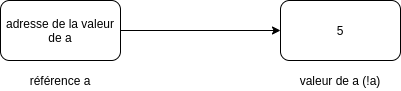
\includegraphics[width=300pt]{img/ref.drawio.png} 
\end{figure}

    \textbf{Exercice} : Que valent \texttt{!x} et \texttt{!y} après avoir
exécuté le bout de code suivant? À quoi sert ce code?

\begin{Shaded}
\begin{Highlighting}[]
\KeywordTok{let}\NormalTok{ x = }\DataTypeTok{ref} \DecValTok{5}\NormalTok{;;}
\KeywordTok{let}\NormalTok{ y = }\DataTypeTok{ref} \DecValTok{27}\NormalTok{;;}
\NormalTok{x := !x + !y;}
\NormalTok{y := !x {-} !y;}
\NormalTok{x := !x {-} !y}
\end{Highlighting}
\end{Shaded}

    \begin{tcolorbox}[breakable, size=fbox, boxrule=1pt, pad at break*=1mm,colback=cellbackground, colframe=cellborder]
\prompt{In}{incolor}{35}{\boxspacing}
\begin{Verbatim}[commandchars=\\\{\}]
\PY{k}{let} \PY{n}{x} \PY{o}{=} \PY{n}{ref} \PY{l+m+mi}{5} \PY{k}{in}
\PY{k}{let} \PY{n}{y} \PY{o}{=} \PY{n}{ref} \PY{l+m+mi}{27} \PY{k}{in}
\PY{n}{x} \PY{o}{:=} \PY{o}{!}\PY{n}{x} \PY{o}{+} \PY{o}{!}\PY{n}{y}\PY{o}{;}
\PY{n}{y} \PY{o}{:=} \PY{o}{!}\PY{n}{x} \PY{o}{\PYZhy{}} \PY{o}{!}\PY{n}{y}\PY{o}{;}
\PY{n}{x} \PY{o}{:=} \PY{o}{!}\PY{n}{x} \PY{o}{\PYZhy{}} \PY{o}{!}\PY{n}{y}\PY{o}{;}
\PY{o}{!}\PY{n}{x}\PY{o}{,} \PY{o}{!}\PY{n}{y}\PY{o}{;;} \PY{c}{(*}\PY{c}{ x vaut 27, y vaut 5 : ce bout de code échange les valeurs de x et y }\PY{c}{*)}
\end{Verbatim}
\end{tcolorbox}

            \begin{tcolorbox}[breakable, size=fbox, boxrule=.5pt, pad at break*=1mm, opacityfill=0]
\prompt{Out}{outcolor}{35}{\boxspacing}
\begin{Verbatim}[commandchars=\\\{\}]
- : int * int = (27, 5)

\end{Verbatim}
\end{tcolorbox}
        
    \textbf{Remarque} : utiliser des \texttt{ref} rend souvent le code plus
compliqué, on n'en utilisera que lorsque c'est nécessaire.

    \hypertarget{fonctions}{%
\section{Fonctions}\label{fonctions}}

    \hypertarget{utiliser-une-fonction}{%
\subsection{Utiliser une fonction}\label{utiliser-une-fonction}}

OCaml est un langage fonctionnel, ce qui signifie que : - les fonctions
y occupent une place importante et peuvent être manipulées un peu comme
des variables - les fonctions sont censées ne pas effectuer d'effet de
bord, c'est à dire d'action sur l'extérieur de la fonction (pas de
modification de variable globale, pas d'écriture dans un fichier\ldots)

Pour utiliser une fonction \texttt{f} sur une valeur \texttt{x}, on
écrira simplement \texttt{f\ x} (et non pas \texttt{f(x)}).

Un certain nombre de fonctions sont déjà définies en OCaml. Par exemple,
la racine carrée :

    \begin{tcolorbox}[breakable, size=fbox, boxrule=1pt, pad at break*=1mm,colback=cellbackground, colframe=cellborder]
\prompt{In}{incolor}{1}{\boxspacing}
\begin{Verbatim}[commandchars=\\\{\}]
\PY{n}{sqrt} \PY{l+m+mi}{2}\PY{o}{.}\PY{l+m+mi}{0} \PY{c}{(*}\PY{c}{ renvoie une approximation de racine de 2 }\PY{c}{*)}
\end{Verbatim}
\end{tcolorbox}

            \begin{tcolorbox}[breakable, size=fbox, boxrule=.5pt, pad at break*=1mm, opacityfill=0]
\prompt{Out}{outcolor}{1}{\boxspacing}
\begin{Verbatim}[commandchars=\\\{\}]
- : float = 1.41421356237309515

\end{Verbatim}
\end{tcolorbox}
        
    Chaque fonction possède une \textbf{signature}, qui donne les types des
paramètres (valeurs en entrée de la fonction) et le type de la valeur de
retour.

    \begin{tcolorbox}[breakable, size=fbox, boxrule=1pt, pad at break*=1mm,colback=cellbackground, colframe=cellborder]
\prompt{In}{incolor}{2}{\boxspacing}
\begin{Verbatim}[commandchars=\\\{\}]
\PY{n}{sqrt}
\end{Verbatim}
\end{tcolorbox}

            \begin{tcolorbox}[breakable, size=fbox, boxrule=.5pt, pad at break*=1mm, opacityfill=0]
\prompt{Out}{outcolor}{2}{\boxspacing}
\begin{Verbatim}[commandchars=\\\{\}]
- : float -> float = <fun>

\end{Verbatim}
\end{tcolorbox}
        
    \texttt{float\ -\textgreater{}\ float} signifie que \texttt{sqrt} est
une fonction qui prend un flottant en entrée et renvoie un flottant. On
ne peut donc pas l'appliquer sur un entier :

    \begin{tcolorbox}[breakable, size=fbox, boxrule=1pt, pad at break*=1mm,colback=cellbackground, colframe=cellborder]
\prompt{In}{incolor}{3}{\boxspacing}
\begin{Verbatim}[commandchars=\\\{\}]
\PY{n}{sqrt} \PY{l+m+mi}{2} \PY{c}{(*}\PY{c}{ erreur : on donne un entier à sqrt qui attend un flottant }\PY{c}{*)}
\end{Verbatim}
\end{tcolorbox}

    \begin{Verbatim}[commandchars=\\\{\}, frame=single, framerule=2mm, rulecolor=\color{outerrorbackground}]
File "[3]", line 1, characters 5-6:
1 | sqrt 2 (* erreur : on donne un entier à sqrt qui attend un flottant *)
         \^{}
Error: This expression has type int but an expression was expected of type
         float

    \end{Verbatim}

    \hypertarget{duxe9finir-une-fonction}{%
\subsection{Définir une fonction}\label{duxe9finir-une-fonction}}

    En OCaml, une fonction se définie de la façon suivante :

\begin{Shaded}
\begin{Highlighting}[]
\KeywordTok{let}\NormalTok{ nom\_fonction nom\_argument = ... }
\end{Highlighting}
\end{Shaded}

où \texttt{...} est le corps de la fonction, c'est à dire ce qui est
exécuté lorsqu'on utilise la fonction.

\textbf{La valeur renvoyée par la fonction est celle de la dernière
instruction (pas besoin de \texttt{return})}.

    Définissons par exemple la fonction \(f: x \longmapsto 2x\) :

    \begin{tcolorbox}[breakable, size=fbox, boxrule=1pt, pad at break*=1mm,colback=cellbackground, colframe=cellborder]
\prompt{In}{incolor}{4}{\boxspacing}
\begin{Verbatim}[commandchars=\\\{\}]
\PY{k}{let} \PY{n}{f} \PY{n}{x} \PY{o}{=} \PY{l+m+mi}{2}\PY{o}{*}\PY{n}{x}
\end{Verbatim}
\end{tcolorbox}

            \begin{tcolorbox}[breakable, size=fbox, boxrule=.5pt, pad at break*=1mm, opacityfill=0]
\prompt{Out}{outcolor}{4}{\boxspacing}
\begin{Verbatim}[commandchars=\\\{\}]
val f : int -> int = <fun>

\end{Verbatim}
\end{tcolorbox}
        
    OCaml nous dit que \texttt{f} est de type
\texttt{int\ -\textgreater{}\ int}, ce qui signifie que \texttt{f} prend
un entier en entrée et renvoie un entier en sortie. Ceci est similaire à
la notation mathématique \(f : \mathbb{N} \longrightarrow \mathbb{N}\).

On peut ensuite utiliser \texttt{f} et récupérer la valeur de retour :

    \begin{tcolorbox}[breakable, size=fbox, boxrule=1pt, pad at break*=1mm,colback=cellbackground, colframe=cellborder]
\prompt{In}{incolor}{5}{\boxspacing}
\begin{Verbatim}[commandchars=\\\{\}]
\PY{n}{f} \PY{l+m+mi}{3}
\end{Verbatim}
\end{tcolorbox}

            \begin{tcolorbox}[breakable, size=fbox, boxrule=.5pt, pad at break*=1mm, opacityfill=0]
\prompt{Out}{outcolor}{5}{\boxspacing}
\begin{Verbatim}[commandchars=\\\{\}]
- : int = 6

\end{Verbatim}
\end{tcolorbox}
        
    Notons que \texttt{x} est une variable \textbf{muette} : elle n'existe
qu'à l'intérieur de \texttt{f}, n'a aucun rapport avec une variable
\texttt{x} définie précédemment et la fonction suivante définit
exactement la même fonction :

    \begin{tcolorbox}[breakable, size=fbox, boxrule=1pt, pad at break*=1mm,colback=cellbackground, colframe=cellborder]
\prompt{In}{incolor}{6}{\boxspacing}
\begin{Verbatim}[commandchars=\\\{\}]
\PY{k}{let} \PY{n}{f} \PY{n}{y} \PY{o}{=} \PY{l+m+mi}{2}\PY{o}{*}\PY{n}{y} \PY{c}{(*}\PY{c}{ peu importe le nom de la variable muette y }\PY{c}{*)}
\end{Verbatim}
\end{tcolorbox}

            \begin{tcolorbox}[breakable, size=fbox, boxrule=.5pt, pad at break*=1mm, opacityfill=0]
\prompt{Out}{outcolor}{6}{\boxspacing}
\begin{Verbatim}[commandchars=\\\{\}]
val f : int -> int = <fun>

\end{Verbatim}
\end{tcolorbox}
        
    Maintenant que \texttt{f} est définie, on peut calculer \(f(3)\) :

    \begin{tcolorbox}[breakable, size=fbox, boxrule=1pt, pad at break*=1mm,colback=cellbackground, colframe=cellborder]
\prompt{In}{incolor}{7}{\boxspacing}
\begin{Verbatim}[commandchars=\\\{\}]
\PY{n}{f} \PY{l+m+mi}{3}
\end{Verbatim}
\end{tcolorbox}

            \begin{tcolorbox}[breakable, size=fbox, boxrule=.5pt, pad at break*=1mm, opacityfill=0]
\prompt{Out}{outcolor}{7}{\boxspacing}
\begin{Verbatim}[commandchars=\\\{\}]
- : int = 6

\end{Verbatim}
\end{tcolorbox}
        
    \textbf{Exercice} : définir la fonction
\(f : x \longmapsto \frac{1}{\sqrt{1 + x^2}}\) en OCaml.

    Comme pour les variables, il est possible d'utiliser \texttt{in} pour
spécifier la portée d'une fonction \(g\)

    \begin{tcolorbox}[breakable, size=fbox, boxrule=1pt, pad at break*=1mm,colback=cellbackground, colframe=cellborder]
\prompt{In}{incolor}{8}{\boxspacing}
\begin{Verbatim}[commandchars=\\\{\}]
\PY{k}{let} \PY{n}{g} \PY{n}{x} \PY{o}{=} \PY{n}{x} \PY{o}{+} \PY{l+m+mi}{1} \PY{k}{in}
\PY{n}{g} \PY{l+m+mi}{0}  \PY{c}{(*}\PY{c}{ g est utilisable seulement dans le in }\PY{c}{*)}
\end{Verbatim}
\end{tcolorbox}

            \begin{tcolorbox}[breakable, size=fbox, boxrule=.5pt, pad at break*=1mm, opacityfill=0]
\prompt{Out}{outcolor}{8}{\boxspacing}
\begin{Verbatim}[commandchars=\\\{\}]
- : int = 1

\end{Verbatim}
\end{tcolorbox}
        
    \textbf{Exercice} Donner la valeur de l'expression suivante :

\begin{Shaded}
\begin{Highlighting}[]
\KeywordTok{let}\NormalTok{ h x = f x + }\DecValTok{1} \KeywordTok{in}
\NormalTok{h }\DecValTok{3}
\end{Highlighting}
\end{Shaded}

    \hypertarget{fonctions-anonymes}{%
\subsection{Fonctions anonymes}\label{fonctions-anonymes}}

    Quand on a besoin d'utiliser une fonction une seule fois, on peut
définir une fonction anonyme (sans nom) avec \texttt{fun}. C'est
l'équivalent de \texttt{lambda} en Python.

    \begin{tcolorbox}[breakable, size=fbox, boxrule=1pt, pad at break*=1mm,colback=cellbackground, colframe=cellborder]
\prompt{In}{incolor}{9}{\boxspacing}
\begin{Verbatim}[commandchars=\\\{\}]
\PY{k}{fun} \PY{n}{x} \PY{o}{\PYZhy{}\PYZgt{}} \PY{n}{x}\PY{o}{*}\PY{l+m+mi}{2} \PY{c}{(*}\PY{c}{ définition d\PYZsq{}une fonction anonyme }\PY{c}{*)}
\end{Verbatim}
\end{tcolorbox}

            \begin{tcolorbox}[breakable, size=fbox, boxrule=.5pt, pad at break*=1mm, opacityfill=0]
\prompt{Out}{outcolor}{9}{\boxspacing}
\begin{Verbatim}[commandchars=\\\{\}]
- : int -> int = <fun>

\end{Verbatim}
\end{tcolorbox}
        
    \begin{tcolorbox}[breakable, size=fbox, boxrule=1pt, pad at break*=1mm,colback=cellbackground, colframe=cellborder]
\prompt{In}{incolor}{10}{\boxspacing}
\begin{Verbatim}[commandchars=\\\{\}]
\PY{o}{(}\PY{k}{fun} \PY{n}{x} \PY{o}{\PYZhy{}\PYZgt{}} \PY{n}{x}\PY{o}{*}\PY{l+m+mi}{2}\PY{o}{)} \PY{l+m+mi}{3} \PY{c}{(*}\PY{c}{ applique une fonction anonyme sur la valeur 3 }\PY{c}{*)}
\end{Verbatim}
\end{tcolorbox}

            \begin{tcolorbox}[breakable, size=fbox, boxrule=.5pt, pad at break*=1mm, opacityfill=0]
\prompt{Out}{outcolor}{10}{\boxspacing}
\begin{Verbatim}[commandchars=\\\{\}]
- : int = 6

\end{Verbatim}
\end{tcolorbox}
        
    \textbf{Remarque} : les deux définitions suivantes sont en fait
complètement équivalentes.

\begin{Shaded}
\begin{Highlighting}[]
\KeywordTok{let}\NormalTok{ f x = ...}
\end{Highlighting}
\end{Shaded}

\begin{Shaded}
\begin{Highlighting}[]
\KeywordTok{let}\NormalTok{ f = }\KeywordTok{fun}\NormalTok{ x {-}\textgreater{} ...}
\end{Highlighting}
\end{Shaded}

Par exemple, on peut définir la fonction
\(f : x \longmapsto 2 \sqrt{x}\) comme ceci :

    \begin{tcolorbox}[breakable, size=fbox, boxrule=1pt, pad at break*=1mm,colback=cellbackground, colframe=cellborder]
\prompt{In}{incolor}{11}{\boxspacing}
\begin{Verbatim}[commandchars=\\\{\}]
\PY{k}{let} \PY{n}{f} \PY{o}{=} \PY{k}{fun} \PY{n}{x} \PY{o}{\PYZhy{}\PYZgt{}} \PY{l+m+mi}{2}\PY{o}{.}\PY{l+m+mi}{0}\PY{o}{*}\PY{o}{.}\PY{n}{x}\PY{o}{*}\PY{o}{*}\PY{l+m+mi}{0}\PY{o}{.}\PY{l+m+mi}{5}
\end{Verbatim}
\end{tcolorbox}

            \begin{tcolorbox}[breakable, size=fbox, boxrule=.5pt, pad at break*=1mm, opacityfill=0]
\prompt{Out}{outcolor}{11}{\boxspacing}
\begin{Verbatim}[commandchars=\\\{\}]
val f : float -> float = <fun>

\end{Verbatim}
\end{tcolorbox}
        
    \textbf{Remarque} : On peut aussi définir une fonction avec
\texttt{function\ x\ -\textgreater{}\ ...} mais \texttt{fun} est
légèrement plus simple d'utilisation.

    \hypertarget{fonctions-de-plusieurs-variables}{%
\subsection{Fonctions de plusieurs
variables}\label{fonctions-de-plusieurs-variables}}

    Il est possible de définir des fonctions avec plusieurs paramètres, par
exemple :

    \begin{tcolorbox}[breakable, size=fbox, boxrule=1pt, pad at break*=1mm,colback=cellbackground, colframe=cellborder]
\prompt{In}{incolor}{12}{\boxspacing}
\begin{Verbatim}[commandchars=\\\{\}]
\PY{k}{let} \PY{n}{sum} \PY{n}{x} \PY{n}{y} \PY{o}{=} \PY{n}{x} \PY{o}{+} \PY{n}{y}
\end{Verbatim}
\end{tcolorbox}

            \begin{tcolorbox}[breakable, size=fbox, boxrule=.5pt, pad at break*=1mm, opacityfill=0]
\prompt{Out}{outcolor}{12}{\boxspacing}
\begin{Verbatim}[commandchars=\\\{\}]
val sum : int -> int -> int = <fun>

\end{Verbatim}
\end{tcolorbox}
        
    \begin{tcolorbox}[breakable, size=fbox, boxrule=1pt, pad at break*=1mm,colback=cellbackground, colframe=cellborder]
\prompt{In}{incolor}{13}{\boxspacing}
\begin{Verbatim}[commandchars=\\\{\}]
\PY{n}{sum} \PY{l+m+mi}{3} \PY{l+m+mi}{4} \PY{c}{(*}\PY{c}{ renvoie 3 + 4 }\PY{c}{*)}
\end{Verbatim}
\end{tcolorbox}

            \begin{tcolorbox}[breakable, size=fbox, boxrule=.5pt, pad at break*=1mm, opacityfill=0]
\prompt{Out}{outcolor}{13}{\boxspacing}
\begin{Verbatim}[commandchars=\\\{\}]
- : int = 7

\end{Verbatim}
\end{tcolorbox}
        
    Le type de \texttt{sum} est
\texttt{int\ -\textgreater{}\ int\ -\textgreater{}\ int}, ce qui peut
paraître étrange. C'est équivalent à
\texttt{int\ -\textgreater{}\ (int\ -\textgreater{}\ int)}, ce qui
signifie que \texttt{sum} prend en entier en argument et renvoie une
valeur de type \texttt{int\ -\textgreater{}\ int} (c'est à dire une
fonction).\\
En effet :

    \begin{tcolorbox}[breakable, size=fbox, boxrule=1pt, pad at break*=1mm,colback=cellbackground, colframe=cellborder]
\prompt{In}{incolor}{14}{\boxspacing}
\begin{Verbatim}[commandchars=\\\{\}]
\PY{n}{sum} \PY{l+m+mi}{3}
\end{Verbatim}
\end{tcolorbox}

            \begin{tcolorbox}[breakable, size=fbox, boxrule=.5pt, pad at break*=1mm, opacityfill=0]
\prompt{Out}{outcolor}{14}{\boxspacing}
\begin{Verbatim}[commandchars=\\\{\}]
- : int -> int = <fun>

\end{Verbatim}
\end{tcolorbox}
        
    \texttt{sum\ 3} est une fonction qui prend en argument un entier
\texttt{y} et qui renvoie \texttt{3\ +\ y}, ce qu'on peut vérifier :

    \begin{tcolorbox}[breakable, size=fbox, boxrule=1pt, pad at break*=1mm,colback=cellbackground, colframe=cellborder]
\prompt{In}{incolor}{15}{\boxspacing}
\begin{Verbatim}[commandchars=\\\{\}]
\PY{k}{let} \PY{n}{f} \PY{o}{=} \PY{n}{sum} \PY{l+m+mi}{3} \PY{k}{in} \PY{c}{(*}\PY{c}{ f est une fonction }\PY{c}{*)}
\PY{n}{f} \PY{l+m+mi}{4} \PY{c}{(*}\PY{c}{ renvoie sum 3 4, c\PYZsq{}est à dire 7 }\PY{c}{*)}
\end{Verbatim}
\end{tcolorbox}

            \begin{tcolorbox}[breakable, size=fbox, boxrule=.5pt, pad at break*=1mm, opacityfill=0]
\prompt{Out}{outcolor}{15}{\boxspacing}
\begin{Verbatim}[commandchars=\\\{\}]
- : int = 7

\end{Verbatim}
\end{tcolorbox}
        
    En fait, OCaml transforme automatiquement une fonction de plusieurs
variables en une suite de fonctions à une variable (c'est ce qu'on
appelle la \textbf{curryfication}) :

    \begin{tcolorbox}[breakable, size=fbox, boxrule=1pt, pad at break*=1mm,colback=cellbackground, colframe=cellborder]
\prompt{In}{incolor}{16}{\boxspacing}
\begin{Verbatim}[commandchars=\\\{\}]
\PY{k}{let} \PY{n}{sum} \PY{o}{=} \PY{k}{fun} \PY{n}{x} \PY{o}{\PYZhy{}\PYZgt{}} \PY{o}{(}\PY{k}{fun} \PY{n}{y} \PY{o}{\PYZhy{}\PYZgt{}} \PY{n}{x} \PY{o}{+} \PY{n}{y}\PY{o}{)} \PY{c}{(*}\PY{c}{ OCaml transforme la définition de sum ci\PYZhy{}dessus en celle\PYZhy{}ci }\PY{c}{*)}
\end{Verbatim}
\end{tcolorbox}

            \begin{tcolorbox}[breakable, size=fbox, boxrule=.5pt, pad at break*=1mm, opacityfill=0]
\prompt{Out}{outcolor}{16}{\boxspacing}
\begin{Verbatim}[commandchars=\\\{\}]
val sum : int -> int -> int = <fun>

\end{Verbatim}
\end{tcolorbox}
        
    \begin{tcolorbox}[breakable, size=fbox, boxrule=1pt, pad at break*=1mm,colback=cellbackground, colframe=cellborder]
\prompt{In}{incolor}{17}{\boxspacing}
\begin{Verbatim}[commandchars=\\\{\}]
\PY{o}{(}\PY{n}{sum} \PY{l+m+mi}{2}\PY{o}{)} \PY{l+m+mi}{3}  \PY{c}{(*}\PY{c}{ le calcul effectué par OCaml lorsqu\PYZsq{}on écrit sum 2 3 }\PY{c}{*)}
\end{Verbatim}
\end{tcolorbox}

            \begin{tcolorbox}[breakable, size=fbox, boxrule=.5pt, pad at break*=1mm, opacityfill=0]
\prompt{Out}{outcolor}{17}{\boxspacing}
\begin{Verbatim}[commandchars=\\\{\}]
- : int = 5

\end{Verbatim}
\end{tcolorbox}
        
    La possibilité d'appliquer une fonction seulement sur certains arguments
s'appelle l'\textbf{application partielle} de fonction. C'est un des
avantages d'OCaml par rapport à Python.

    De la même façon, une fonction OCaml à 3 arguments sera de type
\texttt{...\ -\textgreater{}\ ...\ -\textgreater{}\ ...\ -\textgreater{}\ ...}.

    \textbf{Exercice} : Écrire une fonction
\texttt{delta\ :\ float\ -\textgreater{}\ float\ -\textgreater{}\ float\ -\textgreater{}\ float}
telle que \texttt{delta\ a\ b\ c} renvoie le discriminant de l'équation
\(ax^2 + bx + c = 0\).

    Une fonction peut aussi avoir aucune valeur en entrée. Dans ce cas, on
lui donne l'argument \texttt{()} (de type unit). C'est le cas par
exemple de \texttt{print\_newline}, qui saute une ligne :

    \begin{tcolorbox}[breakable, size=fbox, boxrule=1pt, pad at break*=1mm,colback=cellbackground, colframe=cellborder]
\prompt{In}{incolor}{18}{\boxspacing}
\begin{Verbatim}[commandchars=\\\{\}]
\PY{n}{print\PYZus{}int} \PY{l+m+mi}{0}\PY{o}{;}
\PY{n}{print\PYZus{}newline} \PY{n+nb+bp}{()}\PY{o}{;}
\PY{n}{print\PYZus{}int} \PY{l+m+mi}{1}\PY{o}{;}
\PY{n}{print\PYZus{}newline} \PY{n+nb+bp}{()}\PY{o}{;}
\end{Verbatim}
\end{tcolorbox}

    \begin{Verbatim}[commandchars=\\\{\}]
0
1
    \end{Verbatim}

            \begin{tcolorbox}[breakable, size=fbox, boxrule=.5pt, pad at break*=1mm, opacityfill=0]
\prompt{Out}{outcolor}{18}{\boxspacing}
\begin{Verbatim}[commandchars=\\\{\}]
- : unit = ()

\end{Verbatim}
\end{tcolorbox}
        
    \hypertarget{polymorphisme}{%
\subsection{Polymorphisme}\label{polymorphisme}}

    Reprenons notre 1er exemple de fonction :

    \begin{tcolorbox}[breakable, size=fbox, boxrule=1pt, pad at break*=1mm,colback=cellbackground, colframe=cellborder]
\prompt{In}{incolor}{19}{\boxspacing}
\begin{Verbatim}[commandchars=\\\{\}]
\PY{k}{let} \PY{n}{f} \PY{n}{x} \PY{o}{=} \PY{l+m+mi}{2}\PY{o}{*}\PY{n}{x}
\end{Verbatim}
\end{tcolorbox}

            \begin{tcolorbox}[breakable, size=fbox, boxrule=.5pt, pad at break*=1mm, opacityfill=0]
\prompt{Out}{outcolor}{19}{\boxspacing}
\begin{Verbatim}[commandchars=\\\{\}]
val f : int -> int = <fun>

\end{Verbatim}
\end{tcolorbox}
        
    OCaml sait que l'argument \texttt{x} de \texttt{f} est un \texttt{int}
car on utilise l'opérateur \texttt{*} qui ne s'utilise que sur des
entiers. Mais dans certaines fonctions, il n'y a pas de contrainte de
type :

    \begin{tcolorbox}[breakable, size=fbox, boxrule=1pt, pad at break*=1mm,colback=cellbackground, colframe=cellborder]
\prompt{In}{incolor}{20}{\boxspacing}
\begin{Verbatim}[commandchars=\\\{\}]
\PY{k}{let} \PY{n}{id} \PY{n}{x} \PY{o}{=} \PY{n}{x}
\end{Verbatim}
\end{tcolorbox}

            \begin{tcolorbox}[breakable, size=fbox, boxrule=.5pt, pad at break*=1mm, opacityfill=0]
\prompt{Out}{outcolor}{20}{\boxspacing}
\begin{Verbatim}[commandchars=\\\{\}]
val id : 'a -> 'a = <fun>

\end{Verbatim}
\end{tcolorbox}
        
    Cette fonction \texttt{id} (pour identité) renvoie son argument sans le
modifier. Comme aucune opération n'est appliquée sur \texttt{x}, il n'y
a pas de contrainte sur son type. OCaml utilise alors
\texttt{\textquotesingle{}a} pour désigner le type quelconque de
\texttt{x}.\\
Notons que le type de retour de \texttt{id} est
\texttt{\textquotesingle{}a} également : OCaml nous dit que \texttt{id}
renvoie une valeur du même type que l'argument.

    \textbf{Exercice} : donner le type des fonctions suivantes

\begin{Shaded}
\begin{Highlighting}[]
 \KeywordTok{let}\NormalTok{ f x = }\DecValTok{42}
\end{Highlighting}
\end{Shaded}

\begin{Shaded}
\begin{Highlighting}[]
 \KeywordTok{let}\NormalTok{ f x y = y}
\end{Highlighting}
\end{Shaded}

\begin{Shaded}
\begin{Highlighting}[]
 \KeywordTok{let}\NormalTok{ g x y f = x + f y}
\end{Highlighting}
\end{Shaded}

    \hypertarget{fonction-comme-argument}{%
\subsection{Fonction comme argument}\label{fonction-comme-argument}}

Il est possible d'utiliser une fonction en argument d'une autre
fonction. Par exemple, la fonction suivante évalue une autre fonction en
la valeur 0 :

    \begin{tcolorbox}[breakable, size=fbox, boxrule=1pt, pad at break*=1mm,colback=cellbackground, colframe=cellborder]
\prompt{In}{incolor}{21}{\boxspacing}
\begin{Verbatim}[commandchars=\\\{\}]
\PY{k}{let} \PY{n}{eval} \PY{n}{f} \PY{o}{=}
\PY{n}{f} \PY{l+m+mi}{0}
\end{Verbatim}
\end{tcolorbox}

            \begin{tcolorbox}[breakable, size=fbox, boxrule=.5pt, pad at break*=1mm, opacityfill=0]
\prompt{Out}{outcolor}{21}{\boxspacing}
\begin{Verbatim}[commandchars=\\\{\}]
val eval : (int -> 'a) -> 'a = <fun>

\end{Verbatim}
\end{tcolorbox}
        
    \begin{tcolorbox}[breakable, size=fbox, boxrule=1pt, pad at break*=1mm,colback=cellbackground, colframe=cellborder]
\prompt{In}{incolor}{22}{\boxspacing}
\begin{Verbatim}[commandchars=\\\{\}]
\PY{k}{let} \PY{n}{f} \PY{n}{x} \PY{o}{=} \PY{l+m+mi}{3}\PY{o}{*}\PY{n}{x} \PY{o}{+} \PY{l+m+mi}{7} \PY{k}{in}
\PY{n}{eval} \PY{n}{f}
\end{Verbatim}
\end{tcolorbox}

            \begin{tcolorbox}[breakable, size=fbox, boxrule=.5pt, pad at break*=1mm, opacityfill=0]
\prompt{Out}{outcolor}{22}{\boxspacing}
\begin{Verbatim}[commandchars=\\\{\}]
- : int = 7

\end{Verbatim}
\end{tcolorbox}
        
    \textbf{Exercice} : 1. On définit une fonction \texttt{h} :

\begin{Shaded}
\begin{Highlighting}[]
\KeywordTok{let}\NormalTok{ h f g x = f (g x)}
\end{Highlighting}
\end{Shaded}

Donner la valeur de l'expression :

\begin{Shaded}
\begin{Highlighting}[]
\NormalTok{h (}\KeywordTok{fun}\NormalTok{ x {-}\textgreater{} x*x) (}\KeywordTok{fun}\NormalTok{ x {-}\textgreater{} x + }\DecValTok{1}\NormalTok{) }\DecValTok{3}
\end{Highlighting}
\end{Shaded}

\begin{enumerate}
\def\labelenumi{\arabic{enumi}.}
\setcounter{enumi}{1}
\tightlist
\item
  Donner le type de \texttt{h}.
\item
  À quoi sert \texttt{h}? Comment cette opération s'appelle-t-elle
  mathématiquement?
\end{enumerate}

    \hypertarget{variable-locale-uxe0-une-fonction}{%
\subsection{Variable locale à une
fonction}\label{variable-locale-uxe0-une-fonction}}

    Il est possible de définir une variable dans une fonction :

    \begin{tcolorbox}[breakable, size=fbox, boxrule=1pt, pad at break*=1mm,colback=cellbackground, colframe=cellborder]
\prompt{In}{incolor}{23}{\boxspacing}
\begin{Verbatim}[commandchars=\\\{\}]
\PY{k}{let} \PY{n}{pow4} \PY{n}{x} \PY{o}{=} \PY{c}{(*}\PY{c}{ je saute une ligne ici pour plus de lisibilité }\PY{c}{*)}
    \PY{k}{let} \PY{n}{y} \PY{o}{=} \PY{n}{x}\PY{o}{*}\PY{n}{x} \PY{k}{in}  \PY{c}{(*}\PY{c}{ y est utilisable seulement dans pow4 }\PY{c}{*)}
    \PY{n}{y}\PY{o}{*}\PY{n}{y} \PY{c}{(*}\PY{c}{ renvoie x puissance 4 }\PY{c}{*)}
\end{Verbatim}
\end{tcolorbox}

            \begin{tcolorbox}[breakable, size=fbox, boxrule=.5pt, pad at break*=1mm, opacityfill=0]
\prompt{Out}{outcolor}{23}{\boxspacing}
\begin{Verbatim}[commandchars=\\\{\}]
val pow4 : int -> int = <fun>

\end{Verbatim}
\end{tcolorbox}
        
    \begin{tcolorbox}[breakable, size=fbox, boxrule=1pt, pad at break*=1mm,colback=cellbackground, colframe=cellborder]
\prompt{In}{incolor}{24}{\boxspacing}
\begin{Verbatim}[commandchars=\\\{\}]
\PY{n}{pow4} \PY{l+m+mi}{2} \PY{c}{(*}\PY{c}{ test de notre fonction }\PY{c}{*)}
\end{Verbatim}
\end{tcolorbox}

            \begin{tcolorbox}[breakable, size=fbox, boxrule=.5pt, pad at break*=1mm, opacityfill=0]
\prompt{Out}{outcolor}{24}{\boxspacing}
\begin{Verbatim}[commandchars=\\\{\}]
- : int = 16

\end{Verbatim}
\end{tcolorbox}
        
    On peut aussi définir une fonction à l'intérieur d'une fonction. Par
exemple, on peut définir \(f: x \longmapsto 2x + \sqrt{2(x + 1)}\) en
utilisant une fonction locale \(g : y \longmapsto 2y\) :

    \begin{tcolorbox}[breakable, size=fbox, boxrule=1pt, pad at break*=1mm,colback=cellbackground, colframe=cellborder]
\prompt{In}{incolor}{25}{\boxspacing}
\begin{Verbatim}[commandchars=\\\{\}]
\PY{k}{let} \PY{n}{f} \PY{n}{x} \PY{o}{=} 
    \PY{k}{let} \PY{n}{g} \PY{n}{y} \PY{o}{=} \PY{l+m+mi}{2}\PY{o}{.}\PY{o}{*}\PY{o}{.}\PY{n}{y} \PY{k}{in} \PY{c}{(*}\PY{c}{ g n\PYZsq{}est utilisable que dans f }\PY{c}{*)}
    \PY{n}{g} \PY{n}{x} \PY{o}{+}\PY{o}{.} \PY{o}{(}\PY{n}{g} \PY{o}{(}\PY{n}{x} \PY{o}{+}\PY{o}{.} \PY{l+m+mi}{1}\PY{o}{.}\PY{o}{)}\PY{o}{)}\PY{o}{*}\PY{o}{*}\PY{l+m+mi}{0}\PY{o}{.}\PY{l+m+mi}{5}
\end{Verbatim}
\end{tcolorbox}

            \begin{tcolorbox}[breakable, size=fbox, boxrule=.5pt, pad at break*=1mm, opacityfill=0]
\prompt{Out}{outcolor}{25}{\boxspacing}
\begin{Verbatim}[commandchars=\\\{\}]
val f : float -> float = <fun>

\end{Verbatim}
\end{tcolorbox}
        
    \begin{tcolorbox}[breakable, size=fbox, boxrule=1pt, pad at break*=1mm,colback=cellbackground, colframe=cellborder]
\prompt{In}{incolor}{26}{\boxspacing}
\begin{Verbatim}[commandchars=\\\{\}]
\PY{n}{f} \PY{l+m+mi}{1}\PY{o}{.}
\end{Verbatim}
\end{tcolorbox}

            \begin{tcolorbox}[breakable, size=fbox, boxrule=.5pt, pad at break*=1mm, opacityfill=0]
\prompt{Out}{outcolor}{26}{\boxspacing}
\begin{Verbatim}[commandchars=\\\{\}]
- : float = 4.

\end{Verbatim}
\end{tcolorbox}
        
    \textbf{Exercice} : Écrire une fonction \texttt{swap} qui échange les
valeurs de 2 références en argument.\\
\texttt{swap} doit être de type
\texttt{\textquotesingle{}a\ ref\ -\textgreater{}\ \textquotesingle{}a\ ref\ -\textgreater{}\ unit},
ce qui signifie que \texttt{swap} a deux références en argument, sur des
valeurs de même type \texttt{\textquotesingle{}a}, et ne renvoie pas de
valeur.\\
On rappelle les opérations sur les références :\\
- Définir une référence (locale) : \texttt{let\ a\ =\ ref\ 5\ in\ ...} -
Obtenir la valeur d'une référence : \texttt{!a} - Modifier une référence
: \texttt{a\ :=\ 7}

\textbf{Remarque importante} : Lorsque l'on modifie une référence (ou un
autre objet impératif, comme un tableau) qui est l'argument d'une
fonction, on la modifie aussi à l'extérieur de la fonction. C'est ce
qu'on appelle un \textbf{passage par référence}.

    \hypertarget{booluxe9ens}{%
\subsection{Booléens}\label{booluxe9ens}}

    Une valeur booléenne (bool) est soit true (vrai) soit false (faux).
Exemple de variable de type bool :

    \begin{tcolorbox}[breakable, size=fbox, boxrule=1pt, pad at break*=1mm,colback=cellbackground, colframe=cellborder]
\prompt{In}{incolor}{1}{\boxspacing}
\begin{Verbatim}[commandchars=\\\{\}]
\PY{k}{let} \PY{n}{a} \PY{o}{=} \PY{n+nb+bp}{true}
\end{Verbatim}
\end{tcolorbox}

            \begin{tcolorbox}[breakable, size=fbox, boxrule=.5pt, pad at break*=1mm, opacityfill=0]
\prompt{Out}{outcolor}{1}{\boxspacing}
\begin{Verbatim}[commandchars=\\\{\}]
val a : bool = true

\end{Verbatim}
\end{tcolorbox}
        
    \hypertarget{comparaison}{%
\subsection{Comparaison}\label{comparaison}}

    On peut tester l'égalité de deux \textbf{valeurs} avec \texttt{=} :

    \begin{tcolorbox}[breakable, size=fbox, boxrule=1pt, pad at break*=1mm,colback=cellbackground, colframe=cellborder]
\prompt{In}{incolor}{2}{\boxspacing}
\begin{Verbatim}[commandchars=\\\{\}]
\PY{l+m+mi}{3} \PY{o}{=} \PY{l+m+mi}{1} \PY{o}{+} \PY{l+m+mi}{2}
\end{Verbatim}
\end{tcolorbox}

            \begin{tcolorbox}[breakable, size=fbox, boxrule=.5pt, pad at break*=1mm, opacityfill=0]
\prompt{Out}{outcolor}{2}{\boxspacing}
\begin{Verbatim}[commandchars=\\\{\}]
- : bool = true

\end{Verbatim}
\end{tcolorbox}
        
    On peut aussi utiliser \texttt{=} sur des variables, auquel cas on
compare leurs valeurs :

    \begin{tcolorbox}[breakable, size=fbox, boxrule=1pt, pad at break*=1mm,colback=cellbackground, colframe=cellborder]
\prompt{In}{incolor}{3}{\boxspacing}
\begin{Verbatim}[commandchars=\\\{\}]
\PY{k}{let} \PY{n}{a} \PY{o}{=} \PY{l+m+mi}{3} \PY{k}{in}
\PY{k}{let} \PY{n}{b} \PY{o}{=} \PY{l+m+mi}{4} \PY{k}{in}
\PY{n}{a} \PY{o}{=} \PY{n}{b} \PY{c}{(*}\PY{c}{ teste si les valeurs de a et b sont égales }\PY{c}{*)}
\end{Verbatim}
\end{tcolorbox}

            \begin{tcolorbox}[breakable, size=fbox, boxrule=.5pt, pad at break*=1mm, opacityfill=0]
\prompt{Out}{outcolor}{3}{\boxspacing}
\begin{Verbatim}[commandchars=\\\{\}]
- : bool = false

\end{Verbatim}
\end{tcolorbox}
        
    \textbf{Attention} : le \texttt{=} de OCaml correspond au \texttt{==} de
Python. \texttt{==} existe en OCaml, mais compare les \textbf{adresses
mémoires} de 2 variables au lieu de leurs valeurs et on ne l'utilisera
presque jamais.

    On peut comparer des valeurs numériques avec \texttt{\textless{}}
(inférieur strict), \texttt{\textgreater{}}, \texttt{\textless{}=}
(inférieur ou égal), \texttt{\textgreater{}=},
\texttt{\textless{}\textgreater{}} (différent)\ldots{} :

    \begin{tcolorbox}[breakable, size=fbox, boxrule=1pt, pad at break*=1mm,colback=cellbackground, colframe=cellborder]
\prompt{In}{incolor}{4}{\boxspacing}
\begin{Verbatim}[commandchars=\\\{\}]
\PY{l+m+mi}{2} \PY{o}{\PYZlt{}} \PY{l+m+mi}{1}
\end{Verbatim}
\end{tcolorbox}

            \begin{tcolorbox}[breakable, size=fbox, boxrule=.5pt, pad at break*=1mm, opacityfill=0]
\prompt{Out}{outcolor}{4}{\boxspacing}
\begin{Verbatim}[commandchars=\\\{\}]
- : bool = false

\end{Verbatim}
\end{tcolorbox}
        
    Il faut obligatoirement comparer des valeurs de même type :

    \begin{tcolorbox}[breakable, size=fbox, boxrule=1pt, pad at break*=1mm,colback=cellbackground, colframe=cellborder]
\prompt{In}{incolor}{5}{\boxspacing}
\begin{Verbatim}[commandchars=\\\{\}]
\PY{l+m+mi}{2}\PY{o}{.}\PY{l+m+mi}{4} \PY{o}{\PYZlt{}} \PY{l+m+mi}{3} \PY{c}{(*}\PY{c}{ on ne peut pas comparer un float avec un int }\PY{c}{*)}
\end{Verbatim}
\end{tcolorbox}

    \begin{Verbatim}[commandchars=\\\{\}, frame=single, framerule=2mm, rulecolor=\color{outerrorbackground}]
File "[5]", line 1, characters 6-7:
1 | 2.4 < 3 (* on ne peut pas comparer un float avec un int *)
          \^{}
Error: This expression has type int but an expression was expected of type
         float

    \end{Verbatim}

    \begin{tcolorbox}[breakable, size=fbox, boxrule=1pt, pad at break*=1mm,colback=cellbackground, colframe=cellborder]
\prompt{In}{incolor}{6}{\boxspacing}
\begin{Verbatim}[commandchars=\\\{\}]
\PY{l+m+mi}{2}\PY{o}{.}\PY{l+m+mi}{4} \PY{o}{\PYZlt{}} \PY{l+m+mi}{3}\PY{o}{.}\PY{l+m+mi}{0} \PY{c}{(*}\PY{c}{ par contre ceci fonctionne }\PY{c}{*)}
\end{Verbatim}
\end{tcolorbox}

            \begin{tcolorbox}[breakable, size=fbox, boxrule=.5pt, pad at break*=1mm, opacityfill=0]
\prompt{Out}{outcolor}{6}{\boxspacing}
\begin{Verbatim}[commandchars=\\\{\}]
- : bool = true

\end{Verbatim}
\end{tcolorbox}
        
    \textbf{Remarque} : pas besoin de mettre des points (.) sur
\texttt{\textless{}}, \texttt{\textgreater{}} \ldots{}

    Les opérateurs \texttt{\&\&} (et), \texttt{\textbar{}\textbar{}} (ou),
\texttt{not} permettent de combiner des conditions :

    \begin{tcolorbox}[breakable, size=fbox, boxrule=1pt, pad at break*=1mm,colback=cellbackground, colframe=cellborder]
\prompt{In}{incolor}{7}{\boxspacing}
\begin{Verbatim}[commandchars=\\\{\}]
\PY{l+m+mi}{1} \PY{o}{\PYZlt{}} \PY{l+m+mi}{2} \PY{o}{\PYZam{}\PYZam{}} \PY{l+m+mi}{2} \PY{o}{\PYZlt{}} \PY{l+m+mi}{3}
\end{Verbatim}
\end{tcolorbox}

            \begin{tcolorbox}[breakable, size=fbox, boxrule=.5pt, pad at break*=1mm, opacityfill=0]
\prompt{Out}{outcolor}{7}{\boxspacing}
\begin{Verbatim}[commandchars=\\\{\}]
- : bool = true

\end{Verbatim}
\end{tcolorbox}
        
    \begin{tcolorbox}[breakable, size=fbox, boxrule=1pt, pad at break*=1mm,colback=cellbackground, colframe=cellborder]
\prompt{In}{incolor}{8}{\boxspacing}
\begin{Verbatim}[commandchars=\\\{\}]
\PY{k}{let} \PY{n}{a} \PY{o}{=} \PY{l+m+mi}{0} \PY{k}{in}
\PY{n}{a} \PY{o}{\PYZlt{}}\PY{o}{\PYZgt{}} \PY{l+m+mi}{0} \PY{o}{|}\PY{o}{|} \PY{n}{a} \PY{o}{\PYZgt{}} \PY{l+m+mi}{3} \PY{c}{(*}\PY{c}{ test si a est différent de 0 ou supérieur à 3 }\PY{c}{*)}
\end{Verbatim}
\end{tcolorbox}

            \begin{tcolorbox}[breakable, size=fbox, boxrule=.5pt, pad at break*=1mm, opacityfill=0]
\prompt{Out}{outcolor}{8}{\boxspacing}
\begin{Verbatim}[commandchars=\\\{\}]
- : bool = false

\end{Verbatim}
\end{tcolorbox}
        
    \textbf{Exercice}

\begin{enumerate}
\def\labelenumi{\arabic{enumi}.}
\tightlist
\item
  Quelle est la valeur du code suivant?
\end{enumerate}

\begin{Shaded}
\begin{Highlighting}[]
\KeywordTok{let}\NormalTok{ a = }\DecValTok{42} \KeywordTok{in}
\DataTypeTok{not}\NormalTok{ (a = }\DecValTok{42}\NormalTok{ \&\& (a \textless{} }\DecValTok{10}\NormalTok{ || a \textgreater{} }\DecValTok{30}\NormalTok{))}
\end{Highlighting}
\end{Shaded}

\begin{enumerate}
\def\labelenumi{\arabic{enumi}.}
\setcounter{enumi}{1}
\tightlist
\item
  Comment aurait-on pu écrire
  \texttt{not\ (a\ =\ 42\ \&\&\ (a\ \textless{}\ 10\ \textbar{}\textbar{}\ a\ \textgreater{}\ 30))}
  sans \texttt{not}?
\item
  Écrire une fonction
  \texttt{xor\ :\ bool\ -\textgreater{}\ bool\ -\textgreater{}\ bool}
  telle que \texttt{xor\ a\ b} renvoie le ``ou exclusif'' de \texttt{a}
  et \texttt{b}, c'est à dire \texttt{true} si \texttt{a} ou \texttt{b}
  est \texttt{true}, mais pas les deux.
\end{enumerate}

    \hypertarget{condition-if}{%
\subsection{Condition if}\label{condition-if}}

On peut écrire une condition \texttt{if} de la façon suivante en OCaml :

\begin{Shaded}
\begin{Highlighting}[]
\KeywordTok{if}\NormalTok{ ... }\KeywordTok{then}\NormalTok{ ... }\KeywordTok{else}\NormalTok{ ...}
\end{Highlighting}
\end{Shaded}

La condition du \texttt{if} doit être un booléen. Si la condition est
vraie, le \texttt{then} est exécuté et sa valeur est renvoyé. Sinon,
c'est la valeur du \texttt{else} qui est renvoyé :

    \begin{tcolorbox}[breakable, size=fbox, boxrule=1pt, pad at break*=1mm,colback=cellbackground, colframe=cellborder]
\prompt{In}{incolor}{9}{\boxspacing}
\begin{Verbatim}[commandchars=\\\{\}]
\PY{k}{if} \PY{l+m+mi}{1} \PY{o}{=} \PY{l+m+mi}{2} \PY{k}{then} \PY{l+m+mi}{42} \PY{k}{else} \PY{l+m+mi}{24}
\end{Verbatim}
\end{tcolorbox}

            \begin{tcolorbox}[breakable, size=fbox, boxrule=.5pt, pad at break*=1mm, opacityfill=0]
\prompt{Out}{outcolor}{9}{\boxspacing}
\begin{Verbatim}[commandchars=\\\{\}]
- : int = 24

\end{Verbatim}
\end{tcolorbox}
        
    Définissons par exemple la fonction valeur absolue
(\(x \longmapsto \vert x \vert\)) :

    \begin{tcolorbox}[breakable, size=fbox, boxrule=1pt, pad at break*=1mm,colback=cellbackground, colframe=cellborder]
\prompt{In}{incolor}{10}{\boxspacing}
\begin{Verbatim}[commandchars=\\\{\}]
\PY{k}{let} \PY{n}{abs} \PY{n}{x} \PY{o}{=}
    \PY{k}{if} \PY{n}{x} \PY{o}{\PYZlt{}} \PY{l+m+mi}{0}\PY{o}{.} \PY{k}{then} \PY{o}{\PYZhy{}.} \PY{n}{x}
    \PY{k}{else} \PY{n}{x}
\end{Verbatim}
\end{tcolorbox}

            \begin{tcolorbox}[breakable, size=fbox, boxrule=.5pt, pad at break*=1mm, opacityfill=0]
\prompt{Out}{outcolor}{10}{\boxspacing}
\begin{Verbatim}[commandchars=\\\{\}]
val abs : float -> float = <fun>

\end{Verbatim}
\end{tcolorbox}
        
    Rappelons qu'il n'y a pas de \texttt{return} en OCaml : c'est la
dernière expression calculée par la fonction qui est renvoyée. Ainsi
\texttt{abs\ x} renvoie \texttt{-x} si \texttt{x} est négatif et
\texttt{x} sinon.

    \begin{tcolorbox}[breakable, size=fbox, boxrule=1pt, pad at break*=1mm,colback=cellbackground, colframe=cellborder]
\prompt{In}{incolor}{11}{\boxspacing}
\begin{Verbatim}[commandchars=\\\{\}]
\PY{n}{abs} \PY{o}{(}\PY{o}{\PYZhy{}}\PY{l+m+mi}{2}\PY{o}{.}\PY{l+m+mi}{718}\PY{o}{)}  \PY{c}{(*}\PY{c}{ je mets des parenthèses à cause du \PYZhy{} }\PY{c}{*)}
\end{Verbatim}
\end{tcolorbox}

            \begin{tcolorbox}[breakable, size=fbox, boxrule=.5pt, pad at break*=1mm, opacityfill=0]
\prompt{Out}{outcolor}{11}{\boxspacing}
\begin{Verbatim}[commandchars=\\\{\}]
- : float = 2.718

\end{Verbatim}
\end{tcolorbox}
        
    Pour plus de lisibilité on sautera une ligne avant \texttt{then} et
\texttt{else}, sauf si le contenu du \texttt{if} est très court.

    Dans un \texttt{if\ ...\ then\ ...\ else\ ...}, les valeurs dans le
\texttt{then} et dans le \texttt{else} doivent être de même type :

    \begin{tcolorbox}[breakable, size=fbox, boxrule=1pt, pad at break*=1mm,colback=cellbackground, colframe=cellborder]
\prompt{In}{incolor}{12}{\boxspacing}
\begin{Verbatim}[commandchars=\\\{\}]
\PY{k}{if} \PY{l+m+mi}{1} \PY{o}{=} \PY{l+m+mi}{1} \PY{k}{then} \PY{l+m+mi}{2}
\PY{k}{else} \PY{l+m+mi}{3}\PY{o}{.}\PY{l+m+mi}{14}  \PY{c}{(*}\PY{c}{ impossible d\PYZsq{}avoir 2 types différents dans le then et else }\PY{c}{*)}
\end{Verbatim}
\end{tcolorbox}

    \begin{Verbatim}[commandchars=\\\{\}, frame=single, framerule=2mm, rulecolor=\color{outerrorbackground}]
File "[12]", line 2, characters 5-9:
2 | else 3.14  (* impossible d'avoir 2 types différents dans le then et else *)
         \^{}\^{}\^{}\^{}
Error: This expression has type float but an expression was expected of type
         int

    \end{Verbatim}

    La valeur renvoyée par \texttt{if\ ...\ then\ ...\ else\ ...} peut être
stockée dans une variable :

    \begin{tcolorbox}[breakable, size=fbox, boxrule=1pt, pad at break*=1mm,colback=cellbackground, colframe=cellborder]
\prompt{In}{incolor}{13}{\boxspacing}
\begin{Verbatim}[commandchars=\\\{\}]
\PY{k}{let} \PY{n}{a} \PY{o}{=} \PY{o}{\PYZhy{}}\PY{l+m+mi}{5} \PY{k}{in}
\PY{k}{let} \PY{n}{b} \PY{o}{=} \PY{k}{if} \PY{n}{a} \PY{o}{\PYZgt{}} \PY{l+m+mi}{0} \PY{k}{then} \PY{n}{a} \PY{k}{else} \PY{o}{\PYZhy{}}\PY{n}{a} \PY{k}{in} \PY{c}{(*}\PY{c}{ on pourrait aussi calculer une valeur absolue comme ça }\PY{c}{*)} 
\PY{n}{b}  \PY{c}{(*}\PY{c}{ b vaut 5 }\PY{c}{*)}
\end{Verbatim}
\end{tcolorbox}

            \begin{tcolorbox}[breakable, size=fbox, boxrule=.5pt, pad at break*=1mm, opacityfill=0]
\prompt{Out}{outcolor}{13}{\boxspacing}
\begin{Verbatim}[commandchars=\\\{\}]
- : int = 5

\end{Verbatim}
\end{tcolorbox}
        
    \textbf{Exercice} Définir les fonctions suivantes en OCaml :\\
1.

\begin{enumerate}
\def\labelenumi{\arabic{enumi}.}
\setcounter{enumi}{1}
\tightlist
\item
\end{enumerate}

\begin{enumerate}
\def\labelenumi{\arabic{enumi}.}
\setcounter{enumi}{2}
\tightlist
\item
\end{enumerate}

    \textbf{Exercice} Écrire une fonction
\texttt{n\_solutions\ :\ float\ -\textgreater{}\ float\ -\textgreater{}\ float\ -\textgreater{}\ int}
telle que \texttt{n\_solutions\ a\ b\ c} renvoie le nombre de solutions
de l'équation \(ax^2 + bx + c\).

    \hypertarget{ruxe9cursivituxe9}{%
\section{Récursivité}\label{ruxe9cursivituxe9}}

La récursivité est la possibilité pour une fonction de s'appeller
soi-même. En général, il y a deux étapes pour écrire une fonction
récursive : 1. Un \textbf{cas de base} où la fonction renvoie
directement une valeur. 2. Un \textbf{cas général} où la fonction
s'appelle sur des paramètres ``plus petits''.

En OCaml, une fonction récursive doit être définie par
\texttt{let\ rec\ ...}. Voici un exemple :

    \begin{tcolorbox}[breakable, size=fbox, boxrule=1pt, pad at break*=1mm,colback=cellbackground, colframe=cellborder]
\prompt{In}{incolor}{1}{\boxspacing}
\begin{Verbatim}[commandchars=\\\{\}]
\PY{k}{let} \PY{k}{rec} \PY{n}{f} \PY{n}{x} \PY{o}{=} \PY{c}{(*}\PY{c}{ exemple de fonction récursive }\PY{c}{*)}
    \PY{k}{if} \PY{n}{x} \PY{o}{=} \PY{l+m+mi}{0} \PY{k}{then} \PY{n}{print\PYZus{}newline} \PY{n+nb+bp}{()} \PY{c}{(*}\PY{c}{ cas de base }\PY{c}{*)}
    \PY{k}{else} \PY{o}{(}\PY{n}{print\PYZus{}int} \PY{n}{x}\PY{o}{;} 
          \PY{n}{f} \PY{o}{(}\PY{n}{x} \PY{o}{\PYZhy{}} \PY{l+m+mi}{1}\PY{o}{)}\PY{o}{)} \PY{c}{(*}\PY{c}{ cas général }\PY{c}{*)}
\end{Verbatim}
\end{tcolorbox}

            \begin{tcolorbox}[breakable, size=fbox, boxrule=.5pt, pad at break*=1mm, opacityfill=0]
\prompt{Out}{outcolor}{1}{\boxspacing}
\begin{Verbatim}[commandchars=\\\{\}]
val f : int -> unit = <fun>

\end{Verbatim}
\end{tcolorbox}
        
    \texttt{f\ x} affiche un retour à la ligne si \texttt{x} est égal à 0,
et sinon affiche \texttt{x} puis appelle \texttt{f\ (x\ -\ 1)}.

    Essayons cette fonction :

    \begin{tcolorbox}[breakable, size=fbox, boxrule=1pt, pad at break*=1mm,colback=cellbackground, colframe=cellborder]
\prompt{In}{incolor}{2}{\boxspacing}
\begin{Verbatim}[commandchars=\\\{\}]
\PY{n}{f} \PY{l+m+mi}{2}
\end{Verbatim}
\end{tcolorbox}

            \begin{tcolorbox}[breakable, size=fbox, boxrule=.5pt, pad at break*=1mm, opacityfill=0]
\prompt{Out}{outcolor}{2}{\boxspacing}
\begin{Verbatim}[commandchars=\\\{\}]
- : unit = ()

\end{Verbatim}
\end{tcolorbox}
        
    \begin{Verbatim}[commandchars=\\\{\}]
21
    \end{Verbatim}

    Voici ce qui se passe lors de cet appel \texttt{f\ 2} :

\begin{enumerate}
\def\labelenumi{\arabic{enumi}.}
\tightlist
\item
  On regarde si \texttt{2\ =\ 0}, ce qui est faux. On passe donc dans le
  \texttt{else}.
\item
  On affiche \texttt{2} avec \texttt{print\_int\ x}.
\item
  On appelle \texttt{f} sur la valeur 1. Le calcul de \texttt{f\ 2} se
  met en pause et on exécute \texttt{f\ 1}. Quand \texttt{f\ 1} sera
  terminé, l'appel de \texttt{f\ 2} continuera et \texttt{f\ 1} sera
  remplacé par sa valeur de retour.
\item
  L'exécution de \texttt{f\ 1} affiche \texttt{1} puis appelle
  \texttt{f\ 0}. Le calcul de \texttt{f\ 1} se met en pause et on
  exécute \texttt{f\ 0}. Quand \texttt{f\ 0} sera terminé, l'appel de
  \texttt{f\ 2} continuera et \texttt{f\ 0} sera remplacé par sa valeur
  de retour.
\item
  \texttt{f\ 0} exécute \texttt{print\_newline\ ()} et s'arrête (en
  renvoyant \texttt{()}).
\item
  L'exécution de \texttt{f\ 1} reprend et \texttt{f\ 1} s'arrête.
\item
  L'exécution de \texttt{f\ 2} reprend et \texttt{f\ 2} s'arrête.
\end{enumerate}

    Vous pouvez visualiser l'exécution d'un code similaire en Python avec
\href{http://www.pythontutor.com/visualize.html\#code=def\%20f\%28n\%29\%3A\%0A\%20\%20\%20\%20if\%20n\%20\%3D\%3D\%200\%3A\%0A\%20\%20\%20\%20\%20\%20\%20\%20return\%0A\%20\%20\%20\%20print\%28n\%29\%0A\%20\%20\%20\%20f\%28n-1\%29\%0A\%0Af\%284\%29\&cumulative=false\&curInstr=0\&heapPrimitives=nevernest\&mode=display\&origin=opt-frontend.js\&py=3\&rawInputLstJSON=\%5B\%5D\&textReferences=false}{Python
Tutor}. Il est important de bien comprendre comment les appels récursifs
s'effectuent.

    Un exemple classique d'utilisation de la récursivité est le calcul de la
factorielle d'un entier \(n\), définie par
\(n! = n \times (n - 1) \times ... \times 2 \times 1\).\\
Pour définir une fonction récursive calculant \(n!\) on a besoin de deux
choses : - \textbf{Cas de base} : si \(n = 0\), on peut renvoyer
directement 1 (par convention \(0! = 1\)), sans appel récursif. -
\textbf{Cas général/récurrence} : si \(n\) est quelconque, il faut
rammener le calcul de \(n!\) à un calcul d'une factorielle plus petite
(de façon à se rapprocher du cas de base). Pour cela, on peut remarquer
que \(n! = n\times (n-1)!\) et donc que calculer \((n-1)!\) permet d'en
déduire \(n!\).\\
On en déduit le code suivant :

    \begin{tcolorbox}[breakable, size=fbox, boxrule=1pt, pad at break*=1mm,colback=cellbackground, colframe=cellborder]
\prompt{In}{incolor}{3}{\boxspacing}
\begin{Verbatim}[commandchars=\\\{\}]
\PY{k}{let} \PY{k}{rec} \PY{n}{fact} \PY{n}{n} \PY{o}{=}
    \PY{k}{if} \PY{n}{n} \PY{o}{=} \PY{l+m+mi}{0} \PY{k}{then} \PY{l+m+mi}{1} \PY{c}{(*}\PY{c}{ par convention 0! = 1 }\PY{c}{*)}
    \PY{k}{else} \PY{n}{n}\PY{o}{*}\PY{n}{fact} \PY{o}{(}\PY{n}{n} \PY{o}{\PYZhy{}} \PY{l+m+mi}{1}\PY{o}{)}
\end{Verbatim}
\end{tcolorbox}

            \begin{tcolorbox}[breakable, size=fbox, boxrule=.5pt, pad at break*=1mm, opacityfill=0]
\prompt{Out}{outcolor}{3}{\boxspacing}
\begin{Verbatim}[commandchars=\\\{\}]
val fact : int -> int = <fun>

\end{Verbatim}
\end{tcolorbox}
        
    \begin{tcolorbox}[breakable, size=fbox, boxrule=1pt, pad at break*=1mm,colback=cellbackground, colframe=cellborder]
\prompt{In}{incolor}{4}{\boxspacing}
\begin{Verbatim}[commandchars=\\\{\}]
\PY{n}{fact} \PY{l+m+mi}{4}
\end{Verbatim}
\end{tcolorbox}

            \begin{tcolorbox}[breakable, size=fbox, boxrule=.5pt, pad at break*=1mm, opacityfill=0]
\prompt{Out}{outcolor}{4}{\boxspacing}
\begin{Verbatim}[commandchars=\\\{\}]
- : int = 24

\end{Verbatim}
\end{tcolorbox}
        
    \textbf{Remarque} : Si on oublie le cas de base (\texttt{if\ n\ =\ 0})
la fonction ne s'arrête jamais (\texttt{fact\ 0} appelerait
\texttt{fact\ (-1)} qui appelerait \texttt{fact\ (-2)} et ainsi de
suite\ldots) !

    Écrire une fonction récursive ressemble beaucoup à écrire une
démonstration mathématiques par récurrence et d'ailleurs on utilisera
souvent une démonstration par récurrence pour démontrer qu'une fonction
récursive est correcte, c'est à dire renvoie bien la bonne valeur.\\
Par exemple, pour démontrer que \texttt{fact} est correcte, on peut
poser l'hypothèse de récurrence :
\[\mathcal{H}(n) : \text{fact } n \text{ renvoie } n!\] Preuve : 1.
\(\mathcal{H}(0)\) est vraie car \texttt{fact\ 0} renvoie 1 et, par
définition, \(0! = 1\). 1. Soit \(n\) un entier strictement positif.
Supposons \(\mathcal{H}(n - 1)\) et montrons \(\mathcal{H}(n)\).\\
Comme \(n > 0\), \texttt{fact\ n} renvoie \texttt{n*fact\ (n\ -\ 1)}.
D'après \(\mathcal{H}(n - 1)\), \texttt{fact\ (n\ -\ 1)} renvoie
\((n - 1)!\). Donc \texttt{fact\ n} renvoie \(n(n - 1)! = n!\), ce qui
démontre \(\mathcal{H}(n)\).\\
D'après le principe de récurrence, \(\mathcal{H}(n)\) est vraie pour
tout \(n \in \mathbb{N}\).

    \textbf{Exercice} : Qu'affiche le code suivant? Le deviner puis exécuter
le code pour vérifier.

\begin{Shaded}
\begin{Highlighting}[]
\KeywordTok{let} \KeywordTok{rec}\NormalTok{ f x =}
    \KeywordTok{if}\NormalTok{ x = }\DecValTok{0} \KeywordTok{then} \DataTypeTok{print\_newline}\NormalTok{ ()}
    \KeywordTok{else}\NormalTok{ (f (x {-} }\DecValTok{1}\NormalTok{);}
          \DataTypeTok{print\_int}\NormalTok{ x) }\KeywordTok{in}
\NormalTok{f }\DecValTok{5}    
\end{Highlighting}
\end{Shaded}

    \textbf{Exercice} : 1. Écrire une fonction récursive pour calculer la
somme des \(n\) premiers entiers \(S(n) = 1 + 2 + ... + (n - 1)\). 2.
Quelle formule connaissez-vous pour calculer \(S(n)\)? En déduire une
autre fonction (non récursive) pour calculer cette valeur. Vérifier sur
des exemples que les deux fonctions donnent la même valeur.

    Une application classique de la récursivité est le calcul des termes
d'une suite récurrente.\\
Par exemple : \[\begin{cases} 
u_{n} = 3u_{n-1} + 2, \text{si } n > 0\\
u_0 = 5
\end{cases}\]

    Cette définition par récurrence se traduit naturellement en fonction
récursive :

    \begin{tcolorbox}[breakable, size=fbox, boxrule=1pt, pad at break*=1mm,colback=cellbackground, colframe=cellborder]
\prompt{In}{incolor}{5}{\boxspacing}
\begin{Verbatim}[commandchars=\\\{\}]
\PY{k}{let} \PY{k}{rec} \PY{n}{u} \PY{n}{n} \PY{o}{=} 
    \PY{k}{if} \PY{n}{n} \PY{o}{=} \PY{l+m+mi}{0} \PY{k}{then} \PY{l+m+mi}{5}
    \PY{k}{else} \PY{l+m+mi}{3}\PY{o}{*}\PY{o}{(}\PY{n}{u} \PY{o}{(}\PY{n}{n} \PY{o}{\PYZhy{}} \PY{l+m+mi}{1}\PY{o}{)}\PY{o}{)} \PY{o}{+} \PY{l+m+mi}{2}
\end{Verbatim}
\end{tcolorbox}

            \begin{tcolorbox}[breakable, size=fbox, boxrule=.5pt, pad at break*=1mm, opacityfill=0]
\prompt{Out}{outcolor}{5}{\boxspacing}
\begin{Verbatim}[commandchars=\\\{\}]
val u : int -> int = <fun>

\end{Verbatim}
\end{tcolorbox}
        
    \begin{tcolorbox}[breakable, size=fbox, boxrule=1pt, pad at break*=1mm,colback=cellbackground, colframe=cellborder]
\prompt{In}{incolor}{6}{\boxspacing}
\begin{Verbatim}[commandchars=\\\{\}]
\PY{n}{u} \PY{l+m+mi}{10}
\end{Verbatim}
\end{tcolorbox}

            \begin{tcolorbox}[breakable, size=fbox, boxrule=.5pt, pad at break*=1mm, opacityfill=0]
\prompt{Out}{outcolor}{6}{\boxspacing}
\begin{Verbatim}[commandchars=\\\{\}]
- : int = 354293

\end{Verbatim}
\end{tcolorbox}
        
    \textbf{Exercice} : calculer \(v_{10}\), où \(v_n\) est définie par
\[\begin{cases} 
v_{n+1} = \sqrt{v_{n}} + 4, \text{si } n > 0\\
v_1 = 5
\end{cases}\]

    Un autre exemple classique est la suite de Fibonacci : \[u_0 = 1\]
\[u_1 = 1\] \[u_n = u_{n - 1} + u_{n - 2}\]

On pourrait l'implémenter de la façon suivante :

    \begin{tcolorbox}[breakable, size=fbox, boxrule=1pt, pad at break*=1mm,colback=cellbackground, colframe=cellborder]
\prompt{In}{incolor}{7}{\boxspacing}
\begin{Verbatim}[commandchars=\\\{\}]
\PY{k}{let} \PY{k}{rec} \PY{n}{fibo} \PY{n}{n} \PY{o}{=}
    \PY{k}{if} \PY{n}{n} \PY{o}{\PYZlt{}}\PY{o}{=} \PY{l+m+mi}{1} \PY{k}{then} \PY{l+m+mi}{1}
    \PY{k}{else} \PY{n}{fibo} \PY{o}{(}\PY{n}{n} \PY{o}{\PYZhy{}} \PY{l+m+mi}{1}\PY{o}{)} \PY{o}{+} \PY{n}{fibo} \PY{o}{(}\PY{n}{n} \PY{o}{\PYZhy{}} \PY{l+m+mi}{2}\PY{o}{)} \PY{k}{in}
\PY{n}{fibo} \PY{l+m+mi}{10}
\end{Verbatim}
\end{tcolorbox}

            \begin{tcolorbox}[breakable, size=fbox, boxrule=.5pt, pad at break*=1mm, opacityfill=0]
\prompt{Out}{outcolor}{7}{\boxspacing}
\begin{Verbatim}[commandchars=\\\{\}]
- : int = 89

\end{Verbatim}
\end{tcolorbox}
        
    \textbf{Attention : cette méthode est très inefficace. Pour s'en
convaincre, regardons visuellement les appels récursifs de fibo :}

\begin{figure} 
\centering 
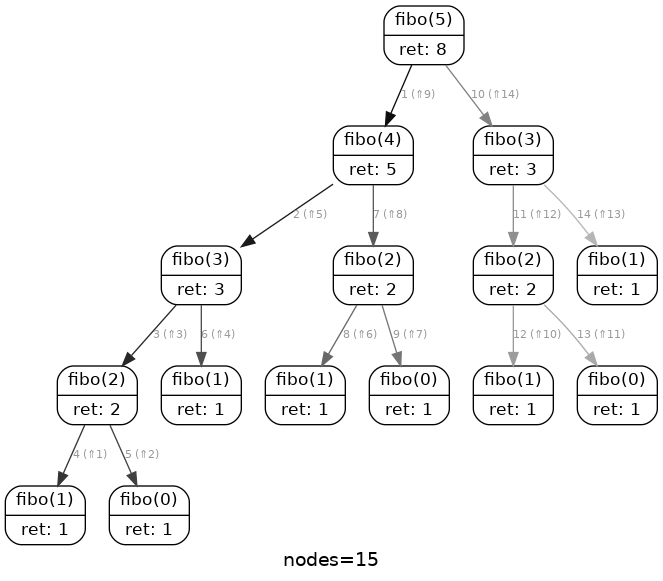
\includegraphics[width=500pt]{img/fibo.png} 
\end{figure}

Il y a de nombreux calculs inutiles : par exemple, \texttt{fibo\ 3} est
appelé 2 fois et \texttt{fibo\ 2} est appelé 3 fois, ce qui est
inefficace.

\textbf{Exercice} : Montrer que le nombre d'appels récursifs pour
calculer \texttt{fibo\ n} est exponentiel en \(n\) (c'est à dire
supérieur à \(a^n\) pour un certain \(a\) indépendant de \(n\)).

Il est possible d'éviter ces appels inutiles en utilisant un
\textbf{accumulateur}. Un accumulateur est un argument d'une fonction
récursive que l'on va utiliser pour construire le résultat final.
L'accumulateur est modifié à chaque appel récursif.

    \begin{tcolorbox}[breakable, size=fbox, boxrule=1pt, pad at break*=1mm,colback=cellbackground, colframe=cellborder]
\prompt{In}{incolor}{8}{\boxspacing}
\begin{Verbatim}[commandchars=\\\{\}]
\PY{k}{let} \PY{k}{rec} \PY{n}{fibo2} \PY{n}{n} \PY{n}{a} \PY{n}{b} \PY{o}{=}
  \PY{k}{if} \PY{n}{n} \PY{o}{=} \PY{l+m+mi}{0} \PY{k}{then} \PY{n}{b}
  \PY{k}{else} \PY{n}{fibo2} \PY{o}{(}\PY{n}{n} \PY{o}{\PYZhy{}} \PY{l+m+mi}{1}\PY{o}{)} \PY{o}{(}\PY{n}{a} \PY{o}{+} \PY{n}{b}\PY{o}{)} \PY{n}{a} \PY{k}{in}
\PY{n}{fibo2} \PY{l+m+mi}{10} \PY{l+m+mi}{1} \PY{l+m+mi}{1}
\end{Verbatim}
\end{tcolorbox}

            \begin{tcolorbox}[breakable, size=fbox, boxrule=.5pt, pad at break*=1mm, opacityfill=0]
\prompt{Out}{outcolor}{8}{\boxspacing}
\begin{Verbatim}[commandchars=\\\{\}]
- : int = 89

\end{Verbatim}
\end{tcolorbox}
        
    On verra aussi plus tard une technique de \textbf{mémoïsation}
permettant d'éviter de faire 2x le même appel récursif, de façon
systématique.

Bien sûr, on pourrait aussi utiliser une boucle \texttt{for} en stockant
les deux derniers termes de la suite dans des variables, mais l'objectif
ici est de s'entraîner à penser récursivement.

    \hypertarget{sous-fonction-ruxe9cursive}{%
\section{Sous-fonction récursive}\label{sous-fonction-ruxe9cursive}}

Quand on souhaite écrire une fonction \texttt{f\ x} en utilisant une
méthode récursive mais que \texttt{x} doit être accessible dans les
appels récursifs, on peut utiliser une sous-fonction récursive dans
\texttt{f}, et \texttt{f} se contentera d'appeler cette fonction.

Par exemple, pour savoir si un entier est premier :

    \begin{tcolorbox}[breakable, size=fbox, boxrule=1pt, pad at break*=1mm,colback=cellbackground, colframe=cellborder]
\prompt{In}{incolor}{9}{\boxspacing}
\begin{Verbatim}[commandchars=\\\{\}]
\PY{k}{let} \PY{n}{premier} \PY{n}{n} \PY{o}{=}
    \PY{k}{let} \PY{k}{rec} \PY{n}{f} \PY{n}{k} \PY{o}{=}  \PY{c}{(*}\PY{c}{ renvoie true si n n\PYZsq{}a pas de diviseurs entre 2 et k }\PY{c}{*)}
        \PY{k}{if} \PY{n}{k} \PY{o}{=} \PY{l+m+mi}{1} \PY{k}{then} \PY{n+nb+bp}{true}  \PY{c}{(*}\PY{c}{ on a regardé tous les diviseurs potentiels }\PY{c}{*)}
        \PY{k}{else} \PY{k}{if} \PY{n}{n} \PY{o+ow}{mod} \PY{n}{k} \PY{o}{=} \PY{l+m+mi}{0} \PY{k}{then} \PY{n+nb+bp}{false}  \PY{c}{(*}\PY{c}{ si k divise n }\PY{c}{*)}
        \PY{k}{else} \PY{n}{f} \PY{o}{(}\PY{n}{k} \PY{o}{\PYZhy{}} \PY{l+m+mi}{1}\PY{o}{)} \PY{k}{in} \PY{c}{(*}\PY{c}{ vérifie que n n\PYZsq{}a pas de diviseurs entre 2 et k }\PY{c}{*)}
    \PY{n}{f} \PY{o}{(}\PY{n}{n} \PY{o}{\PYZhy{}} \PY{l+m+mi}{1}\PY{o}{)}  \PY{c}{(*}\PY{c}{ teste si n a un diviseur entre 2 et n \PYZhy{} 1 }\PY{c}{*)}
\end{Verbatim}
\end{tcolorbox}

            \begin{tcolorbox}[breakable, size=fbox, boxrule=.5pt, pad at break*=1mm, opacityfill=0]
\prompt{Out}{outcolor}{9}{\boxspacing}
\begin{Verbatim}[commandchars=\\\{\}]
val premier : int -> bool = <fun>

\end{Verbatim}
\end{tcolorbox}
        
    \begin{tcolorbox}[breakable, size=fbox, boxrule=1pt, pad at break*=1mm,colback=cellbackground, colframe=cellborder]
\prompt{In}{incolor}{10}{\boxspacing}
\begin{Verbatim}[commandchars=\\\{\}]
\PY{n}{premier} \PY{l+m+mi}{2} \PY{o}{\PYZam{}\PYZam{}} \PY{n}{premier} \PY{l+m+mi}{3} \PY{o}{\PYZam{}\PYZam{}} \PY{n}{not} \PY{o}{(}\PY{n}{premier} \PY{l+m+mi}{4}\PY{o}{)}  \PY{c}{(*}\PY{c}{ test }\PY{c}{*)}
\end{Verbatim}
\end{tcolorbox}

            \begin{tcolorbox}[breakable, size=fbox, boxrule=.5pt, pad at break*=1mm, opacityfill=0]
\prompt{Out}{outcolor}{10}{\boxspacing}
\begin{Verbatim}[commandchars=\\\{\}]
- : bool = true

\end{Verbatim}
\end{tcolorbox}
        
    \begin{tcolorbox}[breakable, size=fbox, boxrule=1pt, pad at break*=1mm,colback=cellbackground, colframe=cellborder]
\prompt{In}{incolor}{ }{\boxspacing}
\begin{Verbatim}[commandchars=\\\{\}]

\end{Verbatim}
\end{tcolorbox}

    Comme en Python, OCaml a deux boucles permettants de répéter des
instructions : \texttt{for} et \texttt{while}.

    \hypertarget{boucle-for}{%
\section{Boucle for}\label{boucle-for}}

Pour répéter \texttt{instructions} pour des valeurs de \texttt{i} allant
de \texttt{a} à \texttt{b} \textbf{inclus} (contrairement à Python) :

\begin{Shaded}
\begin{Highlighting}[]
\KeywordTok{for}\NormalTok{ i=a }\KeywordTok{to}\NormalTok{ b }\KeywordTok{do}
\NormalTok{    instructions}
\KeywordTok{done}
\end{Highlighting}
\end{Shaded}

    \begin{tcolorbox}[breakable, size=fbox, boxrule=1pt, pad at break*=1mm,colback=cellbackground, colframe=cellborder]
\prompt{In}{incolor}{1}{\boxspacing}
\begin{Verbatim}[commandchars=\\\{\}]
\PY{k}{for} \PY{n}{i}\PY{o}{=}\PY{l+m+mi}{0} \PY{k}{to} \PY{l+m+mi}{5} \PY{k}{do}
    \PY{n}{print\PYZus{}int} \PY{n}{i}
\PY{k}{done}\PY{o}{;}
\PY{n}{print\PYZus{}newline}\PY{n+nb+bp}{()}
\end{Verbatim}
\end{tcolorbox}

    \begin{Verbatim}[commandchars=\\\{\}]
012345
    \end{Verbatim}

            \begin{tcolorbox}[breakable, size=fbox, boxrule=.5pt, pad at break*=1mm, opacityfill=0]
\prompt{Out}{outcolor}{1}{\boxspacing}
\begin{Verbatim}[commandchars=\\\{\}]
- : unit = ()

\end{Verbatim}
\end{tcolorbox}
        
    \textbf{Exercice} : Combien de fois est répété
\texttt{for\ i=a\ to\ b\ do\ ...}? (c'est-à-dire : combien y a t-il
d'entiers de \(a\) à \(b\) inclus?)

    \textbf{Exercice} : Écrire une fonction pour calculer la somme des
carrés des \(n\) premiers entiers en utilisant un \texttt{for}, puis une
fonction récursive.

    Comme on le voit sur l'exercice précédent, il est général plus clair et
concis d'écrire une fonction récursive en OCaml. De manière générale, il
ne faut pas abuser des références et boucles et s'entraîner à penser et
écrire récursivement.

    Une variante de la boucle \texttt{for} avec \texttt{downto} permet
d'énumérer ``à l'envers'' :

    \begin{tcolorbox}[breakable, size=fbox, boxrule=1pt, pad at break*=1mm,colback=cellbackground, colframe=cellborder]
\prompt{In}{incolor}{2}{\boxspacing}
\begin{Verbatim}[commandchars=\\\{\}]
\PY{k}{for} \PY{n}{i}\PY{o}{=}\PY{l+m+mi}{5} \PY{k}{downto} \PY{l+m+mi}{0} \PY{k}{do}
    \PY{n}{print\PYZus{}int} \PY{n}{i}
\PY{k}{done}\PY{o}{;}
\PY{n}{print\PYZus{}newline}\PY{n+nb+bp}{()}
\end{Verbatim}
\end{tcolorbox}

    \begin{Verbatim}[commandchars=\\\{\}]
543210
    \end{Verbatim}

            \begin{tcolorbox}[breakable, size=fbox, boxrule=.5pt, pad at break*=1mm, opacityfill=0]
\prompt{Out}{outcolor}{2}{\boxspacing}
\begin{Verbatim}[commandchars=\\\{\}]
- : unit = ()

\end{Verbatim}
\end{tcolorbox}
        
    \hypertarget{boucle-while}{%
\section{Boucle while}\label{boucle-while}}

Pour répéter \texttt{instructions} tant que \texttt{condition} est vraie
:

\begin{Shaded}
\begin{Highlighting}[]
\KeywordTok{while}\NormalTok{ condition }\KeywordTok{do}
\NormalTok{    instructions}
\KeywordTok{done}
\end{Highlighting}
\end{Shaded}

    En guise d'illustration, considérons l'algorithme d'Euclide pour le
calcul du PGCD de deux entiers \(a\) et \(b\). Cet algorithme consiste à
répéter les opérations suivantes tant que \(b \neq 0\) : - Calculer le
reste \(r\) de la division euclidienne de \(a\) par \(b\). - Remplacer
\(a\) par \(b\) et \(b\) par \(r\).

Quand \(b = 0\), on peut montrer que la valeur de \(a\) est le PGCD de
\(a\) et \(b\).

Voici le code OCaml correspondant avec une boucle \texttt{while} :

    \begin{tcolorbox}[breakable, size=fbox, boxrule=1pt, pad at break*=1mm,colback=cellbackground, colframe=cellborder]
\prompt{In}{incolor}{3}{\boxspacing}
\begin{Verbatim}[commandchars=\\\{\}]
\PY{k}{let} \PY{n}{pgcd} \PY{n}{a} \PY{n}{b} \PY{o}{=}
    \PY{k}{let} \PY{n}{q} \PY{o}{=} \PY{n}{ref} \PY{n}{a} \PY{k}{in}
    \PY{k}{let} \PY{n}{r} \PY{o}{=} \PY{n}{ref} \PY{n}{b} \PY{k}{in}
    \PY{k}{while} \PY{o}{!}\PY{n}{r} \PY{o}{\PYZlt{}}\PY{o}{\PYZgt{}} \PY{l+m+mi}{0} \PY{k}{do}
        \PY{k}{let} \PY{n}{tmp} \PY{o}{=} \PY{o}{!}\PY{n}{q} \PY{k}{in} \PY{c}{(*}\PY{c}{ on a besoin de l\PYZsq{}ancienne valeur de q pour calculer le nouveau r }\PY{c}{*)}
        \PY{n}{q} \PY{o}{:=} \PY{o}{!}\PY{n}{r}\PY{o}{;}
        \PY{n}{r} \PY{o}{:=} \PY{n}{tmp} \PY{o+ow}{mod} \PY{o}{!}\PY{n}{r}
    \PY{k}{done}\PY{o}{;}
    \PY{o}{!}\PY{n}{q}\PY{o}{;;}
    
\PY{n}{pgcd} \PY{l+m+mi}{30} \PY{l+m+mi}{12}\PY{o}{;;}
\end{Verbatim}
\end{tcolorbox}

            \begin{tcolorbox}[breakable, size=fbox, boxrule=.5pt, pad at break*=1mm, opacityfill=0]
\prompt{Out}{outcolor}{3}{\boxspacing}
\begin{Verbatim}[commandchars=\\\{\}]
val pgcd : int -> int -> int = <fun>

\end{Verbatim}
\end{tcolorbox}
        
            \begin{tcolorbox}[breakable, size=fbox, boxrule=.5pt, pad at break*=1mm, opacityfill=0]
\prompt{Out}{outcolor}{3}{\boxspacing}
\begin{Verbatim}[commandchars=\\\{\}]
- : int = 6

\end{Verbatim}
\end{tcolorbox}
        
    Voici ce que cela donnerait avec une fonction récursive (encore une fois
c'est beaucoup plus simple en récursif!) :

    \begin{tcolorbox}[breakable, size=fbox, boxrule=1pt, pad at break*=1mm,colback=cellbackground, colframe=cellborder]
\prompt{In}{incolor}{4}{\boxspacing}
\begin{Verbatim}[commandchars=\\\{\}]
\PY{k}{let} \PY{k}{rec} \PY{n}{pgcd} \PY{n}{a} \PY{n}{b} \PY{o}{=}
    \PY{k}{if} \PY{n}{b} \PY{o}{=} \PY{l+m+mi}{0} \PY{k}{then} \PY{n}{a}
    \PY{k}{else} \PY{n}{pgcd} \PY{n}{b} \PY{o}{(}\PY{n}{a} \PY{o+ow}{mod} \PY{n}{b}\PY{o}{)}\PY{o}{;;}

\PY{n}{pgcd} \PY{l+m+mi}{30} \PY{l+m+mi}{12}\PY{o}{;;}
\end{Verbatim}
\end{tcolorbox}

            \begin{tcolorbox}[breakable, size=fbox, boxrule=.5pt, pad at break*=1mm, opacityfill=0]
\prompt{Out}{outcolor}{4}{\boxspacing}
\begin{Verbatim}[commandchars=\\\{\}]
val pgcd : int -> int -> int = <fun>

\end{Verbatim}
\end{tcolorbox}
        
            \begin{tcolorbox}[breakable, size=fbox, boxrule=.5pt, pad at break*=1mm, opacityfill=0]
\prompt{Out}{outcolor}{4}{\boxspacing}
\begin{Verbatim}[commandchars=\\\{\}]
- : int = 6

\end{Verbatim}
\end{tcolorbox}
        
    \textbf{Exercice}\\
Soit \(a \in \mathbb{N}\). La suite de Syracuse est définie par
\(s_0 = a\) et \[s_{n+1} =
\begin{cases} 
     \frac{s_n}{2}, \text{si } n \text{ est pair}\\
    3s_n + 1, \text{sinon}\\
\end{cases}\] Écrire une fonction \texttt{temps\_vol} ayant \(a\) en
argument et renvoyant le premier indice \(n\) tel que \(s_0 = a\) et
\(s_n = 0\).

    \begin{tcolorbox}[breakable, size=fbox, boxrule=1pt, pad at break*=1mm,colback=cellbackground, colframe=cellborder]
\prompt{In}{incolor}{5}{\boxspacing}
\begin{Verbatim}[commandchars=\\\{\}]
\PY{k}{let} \PY{n}{temps\PYZus{}vol} \PY{n}{a} \PY{o}{=} 
    \PY{k}{let} \PY{n}{t} \PY{o}{=} \PY{n}{ref} \PY{l+m+mi}{0} \PY{k}{in}
    \PY{k}{let} \PY{n}{s} \PY{o}{=} \PY{n}{ref} \PY{n}{a} \PY{k}{in}
    \PY{k}{while} \PY{o}{!}\PY{n}{s} \PY{o}{\PYZlt{}}\PY{o}{\PYZgt{}} \PY{l+m+mi}{1} \PY{k}{do}
        \PY{n}{incr} \PY{n}{t}\PY{o}{;}
        \PY{n}{s} \PY{o}{:=} \PY{k}{if} \PY{o}{!}\PY{n}{s} \PY{o+ow}{mod} \PY{l+m+mi}{2} \PY{o}{=} \PY{l+m+mi}{0} \PY{k}{then} \PY{o}{!}\PY{n}{s}\PY{o}{/}\PY{l+m+mi}{2} \PY{k}{else} \PY{l+m+mi}{3}\PY{o}{*} \PY{o}{!}\PY{n}{s} \PY{o}{+} \PY{l+m+mi}{1}
    \PY{k}{done}\PY{o}{;}
    \PY{o}{!}\PY{n}{t} \PY{k}{in}
\PY{n}{temps\PYZus{}vol} \PY{l+m+mi}{10}
\end{Verbatim}
\end{tcolorbox}

            \begin{tcolorbox}[breakable, size=fbox, boxrule=.5pt, pad at break*=1mm, opacityfill=0]
\prompt{Out}{outcolor}{5}{\boxspacing}
\begin{Verbatim}[commandchars=\\\{\}]
- : int = 6

\end{Verbatim}
\end{tcolorbox}
        
    \begin{tcolorbox}[breakable, size=fbox, boxrule=1pt, pad at break*=1mm,colback=cellbackground, colframe=cellborder]
\prompt{In}{incolor}{ }{\boxspacing}
\begin{Verbatim}[commandchars=\\\{\}]

\end{Verbatim}
\end{tcolorbox}


    % Add a bibliography block to the postdoc
    
    
    
\end{document}
